% Based on the supplied springer-template.tex. All manuscript content is here.
\documentclass[pdflatex,sn-mathphys-num]{sn-jnl}
\usepackage[T1]{fontenc}
\usepackage{lmodern}
\usepackage{amsmath,amssymb,amsfonts,amsthm}
\usepackage{graphicx,booktabs,tabularx,multirow}
\usepackage{xcolor,tikz,algorithm,algorithmicx}
\usepackage[noend]{algpseudocode}
\usepackage{listings,enumitem,placeins,needspace,hyperref}
\usepackage[expansion=false]{microtype}
\usepackage{pgfplots,longtable}
\usepgfplotslibrary{groupplots}
\pgfplotsset{compat=1.18,vgcplot/.style={font=\scriptsize,
  label style={font=\small},tick label style={font=\scriptsize},
  axis line style={draw=inkblue!45},tick style={draw=inkblue!35},
  xmajorgrids=true,ymajorgrids=false,grid style={draw=gray!18},
  legend style={font=\scriptsize},clip=false}}
\usetikzlibrary{arrows.meta,positioning,fit,calc,automata}
\hypersetup{colorlinks=true,linkcolor=black,citecolor=black,urlcolor=black,bookmarksdepth=2,pdftitle={A Formal Semantics for Reliable Collaboration among Generative AI Agents in Software Systems},pdfauthor={Majid Babaei}}
\theoremstyle{thmstyleone}
\newtheorem{theorem}{Theorem}
\newtheorem{proposition}[theorem]{Proposition}
\newtheorem{corollary}[theorem]{Corollary}
\theoremstyle{thmstylethree}
\newtheorem{definition}{Definition}
\theoremstyle{thmstyletwo}
\newtheorem{example}{Example}
\newcommand{\Keys}{\mathcal K}
\newcommand{\Jobs}{\mathcal J}
\newcommand{\Sig}{\sigma}
\newcommand{\fresh}{\operatorname{fresh}}
\newcommand{\Pub}{\operatorname{Publishable}}
\newcommand{\obs}{\operatorname{obs}}
\newcommand{\botv}{\perp}
\definecolor{inkblue}{RGB}{31,70,104}
\definecolor{pale}{RGB}{239,245,249}
\definecolor{resultteal}{RGB}{23,130,132}
\definecolor{resultamber}{RGB}{216,126,45}
\tikzset{box/.style={draw=inkblue,rounded corners=2pt,fill=pale,align=center,minimum height=9mm,font=\small},arr/.style={-{Stealth[length=2mm]},thick,draw=inkblue}}
\lstset{basicstyle=\ttfamily\scriptsize,breaklines=true,frame=single,columns=fullflexible,keepspaces=true,showstringspaces=false}
\raggedbottom
\renewcommand{\topfraction}{0.9}
\renewcommand{\bottomfraction}{0.85}
\renewcommand{\textfraction}{0.08}
\renewcommand{\floatpagefraction}{0.75}
\setcounter{topnumber}{4}
\setcounter{bottomnumber}{4}
\setcounter{totalnumber}{6}
\begin{document}
\title[A Formal Semantics for Reliable Collaboration among Generative AI Agents in Software Systems]{A Formal Semantics for Reliable Collaboration among Generative AI Agents in Software Systems}
\author*[1]{\fnm{Majid} \sur{Babaei}}\email{majid.babaei@ufv.ca}
\affil*[1]{\orgdiv{School of Computing},\orgname{University of the Fraser Valley},\orgaddress{\state{BC},\country{Canada}}}
\abstract{Generative workers can propose useful software artifacts without reliably respecting the dependencies, ownership boundaries, and completion conditions of a collaborative workflow. We develop a formal coordination semantics in which workers supply untrusted primitive values (text or code attributes) while a deterministic controller owns artifact structure and publication. Ranked acyclic transformation rules establish persistent correspondences between heterogeneous views. Each generated binding carries an exact dependency signature that includes selected shared context and its generation contract. A guarded transition system separates dispatch, validation, commitment, invalidation, and reconfiguration; a publication barrier checks global consistency. We prove structural integrity, current-contract acceptance, rejection of obsolete responses, dependency-relative repair locality, and a bound on generation attempts per observed dependency episode. For finite acyclic dependency networks, a topological scheduler reaches either a publishable snapshot or explicit failure under stated response and stability assumptions. A simulation theorem relates asynchronous execution to an atomic specification, and transactional configuration changes preserve the safety invariant. Counterexamples delimit the results: incomplete footprints conceal semantic changes, local validators do not imply joint consistency, and bounded retries do not ensure successful generation. Scoped proof-assistant lemmas, bounded state exploration, and a scripted document-service case study exercise the obligations; full controller mechanization and implementation refinement remain open. The resulting guarantees concern coordination and validator-relative correctness; they do not require a probabilistic model of a language model or establish unrestricted functional correctness of generated software.}
\keywords{Runtime enforcement, State machines, Model transformation, Incremental verification, Generative systems, Formal coordination}
\maketitle

\section{Introduction}\label{sec:intro}
A software workflow may distribute requirements, architecture, implementation, and verification among workers with different representations. A requirement is neither an operation signature nor a test oracle. Nevertheless, edits to one can invalidate the others. When a worker produces text or code using a generative model, reliable coordination requires more than a syntactically valid response: the controller must know which source state was used, which target may be written, and whether the resulting collection is ready for publication.

The difficulty is particularly visible during asynchronous execution. Suppose an implementation request is dispatched for requirement revision 1. Revision 2 arrives while generation is running, and the old answer returns later. A parser can accept that answer even though it answers an obsolete question. A second difficulty arises when two answers pass their individual validators but disagree on an interface type. A third arises when a new reviewer is added after the existing workflow appears complete. These failures involve coordination state and can be specified without assuming that a worker reasons correctly.

We study the following question: under which explicit conditions can a controller coordinate arbitrary generative proposals while preserving structural integrity, admitting only current validated values, repairing changes locally, and terminating with an honest completion verdict? Our approach separates deterministic structural transformation from untrusted value proposal. It gives each proposal an identity, a dependency signature, and a bounded attempt episode, meaning one period with unchanged dependencies. Shared knowledge is another versioned dependency. Team changes are atomic transactions over the configuration of the controller.

The formal contribution is a single semantics connecting these mechanisms. First, we define a network of guarded binding automata and a deterministic structural normalizer. Second, we prove invariants and a refinement theorem for asynchronous responses. Third, we characterize locality and finite-episode cost without claiming deterministic generated values. Fourth, we give a sufficient acyclic scheduling discipline for terminality and a safety rule for reconfiguration. Full mathematical proofs appear with their statements. Scoped proof-assistant lemmas, multiple bounded TLC configurations, and a scripted reference controller supply complementary evidence. The central inductive invariant and simulation mechanization remain open.

Runtime enforcement, incremental computation, and model consistency each supply part of the foundation~\cite{schneider,acar,mokhov,stevens}. Our concern is their intersection with proposal rejection, failed-attempt memory, context selection, and changing generation contracts. We do not claim that state machines or dependency tracking are new. The useful distinction is between an accepted value, a currently usable value, and a globally publishable snapshot. Keeping these notions separate prevents several plausible but invalid correctness arguments.

\section{Foundations and running example}\label{sec:found}
\subsection{Formal setting}
A typed view is a finite graph with stable object identities, typed primitive attributes (strings, Booleans, numbers, or inert code text), and typed references. An object identity is retained when one of its feature values changes; a reference identifies another object rather than containing a primitive value. A metamodel specifies allowed types, reference multiplicities, and well-formedness predicates. Let $X$ denote the authoritative source views and immutable shared-context snapshots. A primitive location is an object--feature pair. Collection membership, object existence, ordering when relevant, and absence of a selected context item are observable data; treating only existing attribute values as dependencies would miss additions and deletions.

We use labeled transition systems $(\mathcal S,\mathcal S_0,\Lambda,\longrightarrow)$, consisting of a state set, initial-state set, event labels, and transition relation. A controller state is one element $S\in\mathcal S$. A run is a finite or infinite sequence of labeled transitions from $\mathcal S_0$. An invariant is a predicate true initially and preserved by every transition. Safety means that every finite reachable prefix respects an invariant. Progress properties require separate scheduling and environment hypotheses. Unbounded signatures, object identities, and primitive values make the general system an infinite-state transition system. A finite-control diagram is therefore an automaton schema, not a claim that the unrestricted workflow is a finite-state machine.

For safety, the proposal source is modeled nondeterministically: it can return any value, malformed data, a duplicate answer, or no useful answer. This overapproximates possible language-model outputs and avoids unsupported probability assumptions. Timeout is a controller event with an explicit operational assumption in the progress theorem. Rejection never makes a bad value public. It can, however, prevent successful completion.

\subsection{A heterogeneous workflow}
The running example is a document-service workflow. An intake view contains requests and clauses. A design view contains endpoints. An implementation view contains code patches. A verification view contains checks. An accepted request $s$ creates endpoint $e_s$; each endpoint creates patch $p_s$; each clause $c$ creates check $t_c$. The clause ``an archived document cannot be overwritten'' changes to ``overwriting an archived document returns status 409.'' Status 409 denotes an HTTP conflict response. The patch must be reconsidered even if the endpoint API signature is unchanged.

Figure~\ref{fig:network} shows the dependencies. The patch footprint, the source data made available to its worker, contains both the API signature and the exact relevant clause text. A security context can contribute a path-handling finding to patch and check generation. A reviewer added later obtains a separate view and fresh obligations. This is an illustrative formal instance; no measurements from an existing workflow are used as experimental results here. The executable study in Section~\ref{sec:case-study} uses the concrete binding chain in Table~\ref{tab:bindings}; Figure~\ref{fig:network} is a schematic motivating example.

\begin{figure}[tb]
\centering
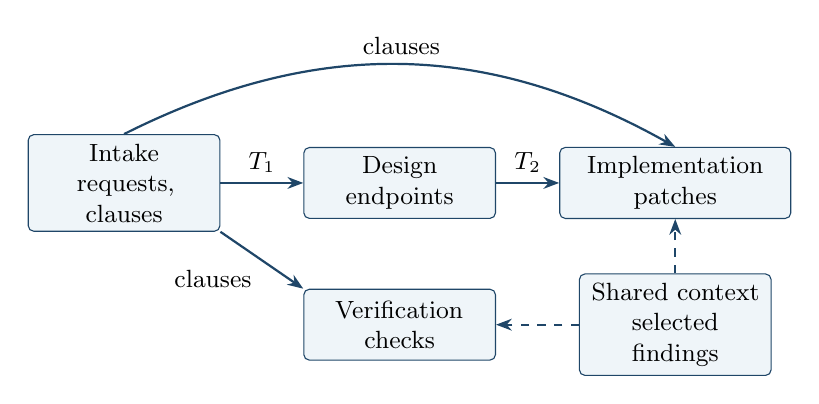
\begin{tikzpicture}
\node[box,text width=22mm] (r) at (0,0) {Intake\\requests, clauses};
\node[box,text width=22mm] (d) at (3.5,0) {Design\\endpoints};
\node[box,text width=27mm] (i) at (7,0) {Implementation\\patches};
\node[box,text width=22mm] (t) at (3.5,-1.8) {Verification\\checks};
\node[box,text width=22mm] (c) at (7,-1.8) {Shared context\\selected findings};
\draw[arr] (r)--node[above,font=\small]{$T_1$}(d);
\draw[arr] (d)--node[above,font=\small]{$T_2$}(i);
\draw[arr] (r.south east)--node[below left,font=\small]{clauses}(t.north west);
\draw[arr] (r.north) to[bend left=28] node[above,font=\small]{clauses}(i.north);
\draw[arr,dashed] (c)--(i);
\draw[arr,dashed] (c)--(t);
\end{tikzpicture}
\caption{A dependency network with heterogeneous views. Solid arrows carry declared source dependencies ($T_1$ derives endpoint interfaces; $T_2$ derives patches); dashed arrows carry selected shared context. The controller constructs objects and references; workers propose primitive attributes}\label{fig:network}
\end{figure}

\section{Transformation contracts and dependency signatures}\label{sec:contracts}
\subsection{Deterministic structure}
A configuration $C$ contains view metamodels, rule definitions, ownership permissions, context policies, validators, generation contracts, and a publication predicate $G$. The base semantics requires a finite ranking of all read dependencies (A0): matches, structural expressions, observations, selectors, and validators may read only external data or strictly earlier stages. This makes availability well defined before progress is considered. A stage groups independent rules/jobs processed after their prerequisites.

A rule has a source tuple pattern, a deterministic guard, one target object, deterministic structural bindings, and zero or more generated primitive bindings. Multi-source matches range over a product of source object sets, rather than an untyped union. Rule identifiers and source identities define the match key
\begin{equation}
q=(r,\operatorname{id}(s_1),\ldots,\operatorname{id}(s_m)).
\end{equation}
For each current match, a deterministic injective constructor produces target identity $\iota(q)$ and persistent trace $q\mapsto\iota(q)$. For example, $(\mathsf{RequestToEndpoint},\mathsf{request17})$ identifies one rule match. Producer namespaces are disjoint ranges of generated identifiers. References resolve through traces only when the referenced match exists. A missing mandatory target makes normalization fail, rather than producing a dangling reference.

Let $N_C$ be the partial structural normalizer over a coherent view snapshot. It is partial because inadmissible candidate snapshots are rejected. It computes the complete current match set for enabled stages $\Keys$, creates missing targets, removes obsolete targets and their owned traces, and computes deterministic attributes and references. It preserves accepted generated values only for surviving target bindings whose contract identity remains compatible. Its range is an internal skeleton: required generated primitive attributes may contain $\botv$, meaning not yet generated. The same symbol later denotes unavailable observations; these are distinct typed uses of an undefined marker. External references to deleted generated objects must be removed, redirected by an explicit rule, or cause normalization failure. Deletion is not presumed harmless.

\begin{definition}[Structural admissibility]\label{def:struct}
Configuration $C$ is structurally admissible on its current view snapshot when $N_C$ terminates, is deterministic (the same snapshot gives the same structure) and idempotent (a second normalization changes nothing), has exactly one owned target and trace per match key, creates only well-typed references, and satisfies all structural multiplicity constraints. Generated bindings may write only declared primitive slots. Every write has one configured owner. A global predicate may impose further constraints beyond these structural conditions.
\end{definition}

This definition is a proof obligation for a concrete transformation engine. We do not infer it for arbitrary transformation programs. A simple sufficient implementation allocates all targets first and resolves references second, using pure guards, disjoint producer namespaces, and total well-typed structural expressions. ATL motivates this allocation/resolution separation~\cite{atl}; unrestricted imperative ATL programs are outside the definition. For dependent stages, normalization reads only usable upstream values; missing upstream values block the dependent stage. Generated values cannot alter their own stage's match set.


\begin{theorem}[A constructive structural kernel]\label{thm:kernel}
Consider finite source graphs and finitely many single-target rules whose guards and structural expressions are pure and terminating. Suppose target identities $\iota(q)$ are injective, producer namespaces are disjoint, primitive expressions have declared types, and each reference expression returns a finite set of current match keys of the required target type and multiplicity. Enumerating matches, allocating all targets, and then resolving references constructs an admissible active skeleton. The result is unique and idempotent when generated slots are held fixed.
\end{theorem}
\begin{proof}
Each source product is finite, so terminating guard evaluation yields a finite match set. Allocation creates one target per key; injectivity and disjoint namespaces exclude collisions. The trace is exactly the graph of $\iota$ restricted to that set. Each reference key is in this domain by hypothesis, so second-phase lookup succeeds and preserves its declared type and cardinality. Typed primitive expressions preserve attribute types. Purity fixes the match set and structural values independently of enumeration order. Repeating the construction uses the same keys, identities, references and values, proving idempotence. Deleting the complement of the current key set gives exactly current coverage, with all references recomputed in the same transaction. Induction over the finite rank order proves the construction for enabled stages.\qedhere
\end{proof}

The key-range and multiplicity conditions are checked on each candidate snapshot. Failure rejects that candidate; the theorem does not require deciding them universally for arbitrary programs. 

If a prerequisite is unavailable, its dependent stage is suspended and contributes no active targets, traces, or jobs. Old accepted pairs remain only in a private cache, unavailable to consumers. Rank-order normalization suspends all affected descendants, so active references never point into suspended stages. On reactivation, stable keys reconstruct objects; cached pairs may be restored only when observation, contract, and authority are compatible. Each reactivated job receives a new episode nonce. A set $Q$ records required suspended stages, preventing empty job sets from being mistaken for completion.

\subsection{What a binding depends on}
Write $j=(q,b)$ for a generated job, consisting of a match key and identifier for one declared generated attribute binding. Let $Z$ be the coherent readable snapshot combining authoritative $X$ and currently usable generated predecessors, constructed from lower to higher rank under A0. Its effective observation is
\begin{equation}\label{eq:obs}
o_j=\obs_{C,j}(Z)=(F_j(Z),\,\operatorname{select}_{C,j}(Z),\,\eta_{C,j}).
\end{equation}
Here $F_j$ is a pure total source-footprint expression, selection includes authorized context items and explicit absence markers, and $\eta_{C,j}$ identifies the complete generation/validation contract. The latter covers the instruction, schema, validator and its environment, source expression, selection policy, and generation settings whose change requires regeneration. A changed configuration need not invalidate every job, but it must change $\eta$ for every affected job.

An API signature such as \texttt{put(id,body)} is an interface attribute. The dependency signature introduced next instead identifies all inputs used to generate an attribute. The signature $\Sig_j=\operatorname{enc}(o_j)$ is an injective canonical encoding: an unambiguous stable serialization in which different observations cannot share an encoding. In the mathematics it is exact equality, not a fixed-length hash. An implementation can store the encoding or use a digest with collision detection; substituting a bare cryptographic digest makes the corresponding results conditional on absence of relevant collisions. Context version numbers are audit information. They enter $o_j$ only if the generator or validator actually observes them. Otherwise equal selected content across different context versions has equal signatures.

Footprints describe dependency functions, not just a list of locations visited on a previous execution. A query ``all findings for endpoint $e$'' depends on the selected set's membership and its contents. Either recomputing that query or maintaining a sound index over its membership dependency is necessary to discover a newly added finding. An access-denied or unavailable required context gives observation $\botv$ and blocks dispatch. Replacing missing context silently with empty text changes the contract.

\begin{definition}[Footprint adequacy]\label{def:adequate}
For a desired Boolean domain relation $R_j(Z,v)$ on readable snapshots and proposed values, a footprint is adequate if there exists $\widehat R_j$ such that $R_j(Z,v)=\widehat R_j(o_j,v)$ for all admissible $Z,v$. A validator $V_j(o,v)$ is sound for that relation if $V_j(o,v)\Rightarrow\widehat R_j(o,v)$.
\end{definition}

In plain language, two snapshots with the same observation must give the same desired-validity judgment for any fixed proposal. Adequacy is a semantic obligation, whereas signature equality is a mechanical test. In the example, a footprint containing only a signature cannot be adequate for a requirement about status 409 when two source states have equal API signatures and different status clauses. No freshness theorem repairs an inadequate specification.

\subsection{Assumptions and guarantees}
Table~\ref{tab:assumptions} collects assumptions used later. They are independently meaningful: disjoint ownership protects writes, exact signatures protect dependency comparison, and sound validation connects acceptance to a domain property. None entails the others.
\begin{table}[tb]
\caption{Assumptions and the guarantees that require them}\label{tab:assumptions}
\small\begin{tabularx}{\linewidth}{@{}lXl@{}}\toprule
ID & Assumption & Used for\\\midrule
A0 & Finite ranked read dependencies; suspension of unavailable stages & Defined semantics\\
A1 & Admissible deterministic normalizer; primitive-only worker writes & Structure\\
A2 & Exact effective signatures; all relevant contract changes included & Freshness, locality\\
A3 & Linearizable controller transactions and immutable observations & Commit safety\\
A4 & Total validators over recorded observations; declared stable environment & Acceptance\\
A5 & Finite acyclic complete dependency graph, single producers, stage stability & Terminality\\
A6 & Inputs/configuration stabilize; controller progresses fairly; requests settle & Progress\\
A7 & Adequate footprints and sound local/global validators & Domain correctness\\\bottomrule
\end{tabularx}
\end{table}

\section{A guarded coordination machine}\label{sec:machine}
\subsection{State and local automata}
The controller state is $S=(C,X,Y,L,B,P,A,H,Q,\nu,\rho)$: configuration, authoritative inputs, active target skeleton, traces, job/cache records, active requests, audit history, optional published snapshot, required suspended stages, fresh-nonce allocator, and semantic revision. At every transition boundary active structure is normalized. A record holds accepted value, stamp, and evidence pointer $(v,a,\gamma)$ or none, failed signature $f$ or none, episode identifier $e$, episode signature $s$, and attempts $n\in\{0,\ldots,k\}$ for fixed $k\geq1$. Evidence $\gamma$ identifies immutable observation, contract, owner, and successful type/validator checks. An episode is a maximal consecutive period with one signature while the job is active; returning to an older signature or reactivating a suspended job starts a new episode. Nonces are allocated monotonically by $\nu$, so request identity $u=(j,e,n)$ is never reused after deletion or recreation.

A request stores immutable $(u,j,e,\Sig,o)$ and its designated owner. At most one request is active for a job episode. Dispatch history is retained in $A$ after a request leaves $P$, allowing late and duplicate deliveries to be recognized. Cancellation prevents commitment; it need not stop remote computation. Attempts count dispatched requests even if they subsequently time out or become obsolete.

Reconciliation is a finite rank-order function. It rebuilds $Q$ from current stage statuses, removing entries for stages that become enabled. An enabled stage with zero matches is settled successfully and is not suspended. At each stage it checks prerequisite usability, suspends unavailable stages and adds them to $Q$, or constructs the stage using the checked kernel. It compares each active job's new signature to its stored episode signature $s$. A difference, new job, or reactivation cancels its request, allocates $e$ from $\nu$, sets $s$ to the new signature, clears $f$, and sets $n=0$. Equal signatures of surviving active jobs preserve counters and evidence. Deletion removes active jobs and cancels requests; historical evidence remains in $A$. Thus no unavailable observation is sent to a worker. Semantic mutations increment $\rho$; currentness of $H$ is derived by comparing its revision to $\rho$.

Let $\Jobs(S)$ contain only active jobs; suspended/cache-only records belong to $B$ but not $\Jobs(S)$. Freshness compares the previously accepted stamp with the current dependency signature. For an active job, define
\begin{align}
\fresh_j(S)&\iff B_j\text{ has }(v,a,\gamma)\ \land\ a=\Sig_j(S),\label{eq:fresh}\\
U_j(S)&\iff j\text{ active}\land\fresh_j(S)\land\bigwedge_{i\prec j}U_i(S),\label{eq:usable}\\
O(S)&=\{j\in\Jobs(S):\neg U_j(S)\}.\label{eq:obligation}
\end{align}
Here $i\prec j$ ranges over declared generated prerequisites; the empty conjunction is true. Evaluate these definitions by rank A0, so they are not cyclic equations. Inactive jobs are unusable. Current validity is deliberately absent from $U$: Theorem~\ref{thm:safety} derives it from acceptance evidence. Validators are total and deterministic on their declared observations; validation involving external tools must include the relevant tool versions and environment in the contract or use an immutable certificate checked against it. A cached historical value may remain for audit, but a downstream consumer may read it only through the $U_j$ gate. If an upstream value is unusable, descendants become unusable as well, even if old bytes are still stored.

Figure~\ref{fig:automaton} summarizes a job's control states. They are derived from record contents; the formal guards below determine the transitions. A dependency change also cancels a Pending request and starts a new episode. The job is Dirty unless compatible cached evidence immediately restores Fresh. Suspension and reactivation are lifecycle operations outside the four local states. The failed state is terminal for an unchanged episode, not a successful accepting state. A worker cannot transition a job directly to fresh.
\begin{figure}[tb]
\centering
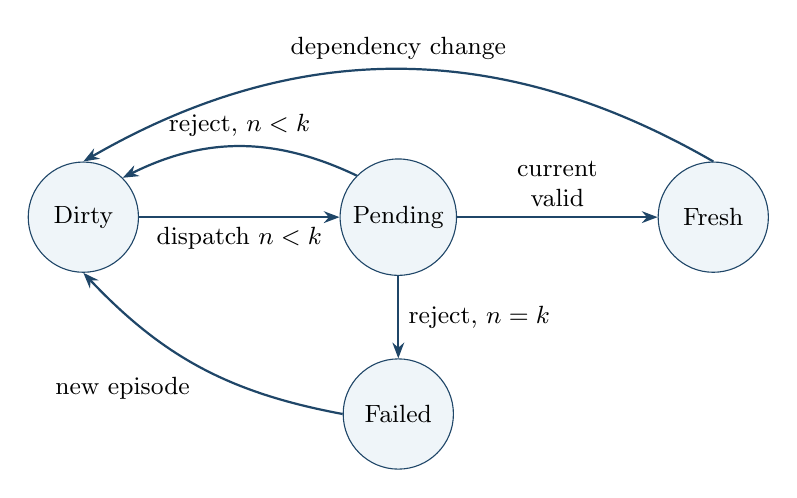
\begin{tikzpicture}[>=Stealth,every state/.style={draw=inkblue,fill=pale,font=\small,minimum size=14mm}]
\node[state] (d) at (0,0) {Dirty};
\node[state] (p) at (4,0) {Pending};
\node[state] (f) at (8,0) {Fresh};
\node[state] (e) at (4,-2.5) {Failed};
\draw[arr] (d) -- node[below,font=\small]{dispatch $n<k$}(p);
\draw[arr] (p) -- node[above,align=center,font=\small]{current\\valid}(f);
\draw[arr] (p.north west) to[bend right=26] node[above,font=\small]{reject, $n<k$}(d.north east);
\draw[arr] (p)--node[right,font=\small]{reject, $n=k$}(e);
\draw[arr] (f.north) to[bend right=30] node[above,font=\small]{dependency change}(d.north);
\draw[arr] (e.west) to[bend left=18] node[below left,font=\small]{new episode}(d.south);
\end{tikzpicture}
\caption{Binding control automaton schema. Dependency changes cancel pending authority and start a new episode; the Fresh-to-Dirty case is illustrated. Compatible historical evidence can instead restore Fresh after reversion or reactivation. Obsolete deliveries cannot write a slot. Suspension removes the active job; reactivation constructs a fresh episode}\label{fig:automaton}
\end{figure}


\begin{table}[tb]
\caption{Key notation for the controller and each generated job}\label{tab:notation}
\small\begin{tabularx}{\linewidth}{@{}lX@{}}\toprule
Symbol & Meaning\\\midrule
$C,X,Y,L$ & Configuration, authoritative input/context, active skeleton, active traces\\
$B,P,A,H$ & Job/cache records, active requests, immutable history/evidence, published snapshot\\
$Q,\nu,\rho$ & Required suspended stages, fresh-nonce allocator, internal semantic revision\\
$j=(q,b)$ & Match key paired with one generated attribute binding\\
$o_j,\Sig_j$ & Current effective observation and its exact encoding\\
$(v,a,\gamma)$ & Accepted value, accepted observation stamp, evidence pointer\\
$(e,s,n,f)$ & Episode nonce, episode signature, attempts, failed signature\\
$U_j,O$ & Current usability and set of active unusable jobs\\\bottomrule
\end{tabularx}
\end{table}
For example, a record may have accepted stamp $a=\Sig_0$ while its episode signature is $s=\Sig_1$ after an edit; it then holds a historical value and requires repair. The nonce $e$ distinguishes this episode from an earlier occurrence of $\Sig_1$. Semantic revision $\rho$ changes on authoritative mutations and need not equal any one source document's version.

\subsection{Transition rules}\label{sec:rules}
Every transition is an atomic controller transaction. Changes to input, structure, and affected job eligibility form one transaction or use a revision barrier that prevents intermediate states from being consumed. We write $S\xrightarrow{\lambda}S'$ for the following rules; all unmentioned components are unchanged.

\paragraph{Edit and normalize.} An authorized edit creates $X'$. Compute $N_C$ on the updated coherent snapshot, update the job set, reconcile signatures and dependent usability, cancel obsolete active requests, and advance $\rho$ so any previous publication becomes historical. If normalization fails, keep the previous coherent state and record the rejected edit. A deletion removes owned jobs and traces and cancels their requests. A later delivery for a nonexistent or recreated job fails the request-identity check.

\paragraph{Dispatch.} For $j\in O(S)$, require current observation $o\ne\botv$, all required upstream jobs usable, no active request, no failed stamp equal to $\Sig_j$, and $n<k$. Increment $n$ and add a request $(u,j,e,\Sig_j,o)$ to $P$. The worker receives only the declared observation and static instruction. The controller records its owner and identity before sending the request.

\paragraph{Resolve and commit.} For a returned $(u,v)$, require $u$ active in $P$, the same existing job and episode, the configured owner still authorized, and, writing $\Sig_u$ for the signature stored in request $u$,
\begin{equation}\label{eq:guard}
\Sig_u=\Sig_j(S),\qquad o_j(S)\ne\botv,\qquad V_j(o_u,v).
\end{equation}
Also require all upstream prerequisites usable and a deterministic type check for the primitive slot. Tentatively install $(v,\Sig_u,\gamma)$ in a private candidate and run complete downstream rank-order normalization and reconciliation, because generated attributes may affect later matches or references. Commit the entire candidate only if all enabled structural checks succeed; otherwise reject it as a failed attempt. A successful commit advances $\rho$, clears failure and removes $u$. Workers supply only primitive proposals; structural changes belong to the controller. 

If the request is active and current but validation, typing, or candidate normalization fails, remove it; at $n=k$ set $f=\Sig_j$, otherwise leave the job eligible. An active current timeout follows the same failure path. An inactive, unauthorized, or obsolete response is discarded; reconciliation already canceled its authority at the associated mutation. Delivery of a duplicate has no effect on semantic state.

The equality test and the slot write must share a linearization point with edits and configuration updates. Testing before acquiring a write lock is insufficient. Validation may run outside the transaction on immutable $o_u$, but its result can be used only after rechecking request activity and Equation~\eqref{eq:guard} inside the transaction. An authentic worker response is not itself evidence that these conditions hold.

\paragraph{Publish.} Let $G(C,X,Y,B,L)$ be a total global predicate evaluated over an immutable candidate snapshot. It includes all mandatory joint constraints and required executable checks. The completion guard below means: no required stage is suspended, no active job is dirty, no active request is pending, and all joint checks pass. Canceled messages still in the network are historical and do not belong to $P$. Set
\begin{equation}\label{eq:publish}
\begin{split}
\Pub(S)\iff{}&\text{structural normal form}\ \land\ Q=\emptyset\\
&{}\land\ O(S)=\emptyset\ \land\ P=\emptyset\ \land\ G(C,X,Y,B,L).
\end{split}
\end{equation}
Only a Publish transition satisfying Equation~\eqref{eq:publish} installs $H$ with that exact snapshot and revision. If $G$ is evaluated outside the transaction, installation compares the candidate revision with current $\rho$ and retries or rejects on mismatch. Its tool environment must be immutable and execution total, just as for local validation. Later edits leave $H$ as a historical snapshot but clear any claim that it represents the current state. Publication means that the specified completion contract holds for that revision.

\paragraph{Configuration transaction.} A candidate $C'$ is checked for structural admissibility, ownership, policy compatibility, contract invalidations, mandatory ranked-read condition A0, and, when progress is required, the additional scheduling discipline of Section~\ref{sec:progress}. Atomically install $C'$, normalize, migrate compatible records, start new episodes for changed signatures, cancel every request whose job, authority, or contract changed, and advance $\rho$, even if only $G$ changed. Reject the entire candidate if any check fails. Reusing a value under a new validator requires revalidation, not merely retaining its previous success bit.

\section{Safety and asynchronous refinement}\label{sec:safety}
\subsection{Inductive safety}
We distinguish a historical acceptance invariant from current usability. A committed value need not remain fresh after an edit. The controller must prevent its use until repaired. Saying that every stored value is always fresh would be false in precisely the change scenarios of interest.

\begin{theorem}[Controller safety]\label{thm:safety}
Under A0--A4, from an initially normalized state with no accepted generated values, every reachable state satisfies: (i) active targets and traces have unique producers and valid structural references; (ii) each accepted record has a recorded authorized successful validation against its recorded observation and contract; (iii) every usable value satisfies the current validator for the current observation; (iv) every committed response was current and authorized at its commit linearization point; and (v) every installed published snapshot satisfied Equation~\eqref{eq:publish} at installation.
\end{theorem}
\begin{proof}
Induct on transition length. Initially (i) is A1 and the remaining claims are vacuous. Edit/normalize preserves (i) by A1 and retains acceptance evidence only as historical records. It recomputes usability, so a changed observation cannot make an old pair usable unless its exact observation and validator contract still agree. Dispatch changes no accepted pair or structure. A successful Resolve tentatively writes the owned primitive slot and normalizes its dependent active structure before admitting the entire candidate; Theorem~\ref{thm:kernel} or A1 establishes (i) for the new active graph, while a rejected candidate leaves it unchanged. Cancellation of suspended jobs preserves request authority; active request identity and authorization establish the provenance part of (ii), and the validator and exact-signature tests establish (iii) and (iv). A failed or discarded response writes no accepted pair. Timeouts change only attempt state. Publish tests the exact snapshot it installs, establishing (v). Configuration transactions normalize under the new admissible configuration, invalidate incompatible evidence, and cancel obsolete authority; they therefore preserve (i)--(iv) and do not relabel a historical publication as current. These are all transitions. In (iii), current equality of the encoded observation implies equality of validator inputs and contract by A2 and A4.\qedhere
\end{proof}

\begin{corollary}[Validator-relative domain correctness]\label{cor:domain}
If a usable accepted value $v$ has an adequate footprint and sound validator in the sense of Definition~\ref{def:adequate}, then $R_j(Z,v)$ holds. If the global predicate is sound for a desired snapshot relation $R_G$, every published snapshot satisfies $R_G$.
\end{corollary}
\begin{proof}
Theorem~\ref{thm:safety}(iii) supplies $V_j(o_j,v)$. Soundness yields $\widehat R_j(o_j,v)$; adequacy identifies it with $R_j(Z,v)$. The second statement applies global soundness to the successful publication guard.\qedhere
\end{proof}

\begin{example}[Limits of parsing and test evidence]\label{ex:limits}
A generated patch returning 200 for every request may parse and type-check while violating the status-409 clause. Such validators are not sound for that clause. A generated test that fails on one empty stub need not detect an incorrect implementation. Similarly, locally accepted endpoints using different document-identifier types can violate a joint interface constraint. The global predicate must check that constraint, or a certified cross-binding validator must cover it. Rejection at the publication barrier is an honest blocked outcome; it is not a proof that automatic repair will succeed.
\end{example}

\subsection{Refinement to atomic accepted updates}
Define an abstract machine $\mathcal A$ whose state consists of configuration, coherent input, structure, accepted records, attempt/failure records, and publication. Its \emph{Accept} transition may choose any proposed value satisfying the current observation's validator and ownership condition and normalize the tentative update using the same checked kernel, and admit it only on success. Its \emph{Attempt} and \emph{Fail} transitions account for budget use and exhaustion; its Edit, Reconfigure, and Publish transitions have the guards above. It has no remote requests. This abstract specification permits many values and schedules; it does not select one canonical generated artifact.

Let $\alpha(S)$ erase requests and audit-delivery detail, retaining the semantic and budget records. Abstract publication drops the concrete requirement $P=\emptyset$, since requests are erased. It therefore permits publication at least whenever the concrete machine does. Concrete dispatch maps to an abstract budget increment, rather than a stutter; claiming that dispatch stutters while retaining an incremented counter would be incorrect.

Table~\ref{tab:abstract} fixes the abstract action relation. Let $s_j$ be the recorded episode signature and $\mathcal R$ the checked rank-order normalization/reconciliation function. Abstract Fail overapproximates failed attempts; it does not infer the existence of an erased request. This specification constrains admitted effects while abstracting the transport protocol.
\begin{table}[tb]
\caption{Abstract action guards and effects; unmentioned fields are unchanged}\label{tab:abstract}
\small\begin{tabularx}{\linewidth}{@{}lXX@{}}\toprule
Action & Guard & Effect\\\midrule
Attempt$(j)$ & Active dirty job, available observation, $n_j<k$, $f_j\ne s_j$ & $n_j\gets n_j+1$\\
Accept$(j,v)$ & Active authorized dirty job, $0<n_j\leq k$, current type/validator checks, candidate normalization succeeds & Install current evidence, clear failure, apply $\mathcal R$\\
Fail$(j)$ & Active dirty job, $0<n_j\leq k$ & If $n_j=k$, set $f_j\gets s_j$\\
Edit / Reconfigure & Authorized candidate passes checked construction & Install candidate, apply $\mathcal R$\\
Publish & Normal form, $Q=O=\emptyset$, $G$ true & Install immutable revision snapshot\\\bottomrule
\end{tabularx}
\end{table}

\begin{theorem}[Forward simulation]\label{thm:refinement}
Under A0--A4, every concrete controller run projects through $\alpha$ to an abstract run, allowing stuttering (an erased step leaves the abstract state unchanged). In particular, asynchronous responses cannot introduce a value forbidden by the atomic accepted-update specification.
\end{theorem}
\begin{proof}
Consider one concrete transition. Dispatch maps to abstract Attempt because both increment the same current-episode budget; request creation is erased. Successful Resolve maps to Accept: the concrete current-signature test implies that its immutable observation is exactly the current abstract observation, and the remaining tests imply the abstract validator and ownership guards. Both actions apply the same checked candidate normalization. Current rejection or timeout maps to Fail, including the exhausted-budget mark if necessary. Obsolete or duplicate delivery changes no retained record and maps to a stutter; signature reconciliation belongs to the associated edit/configuration transition in both machines. Edit and Reconfigure use the same normalized snapshots and migration in both machines. Concrete Publish has all abstract global, structural, and freshness guards, so maps to abstract Publish. Initial projections agree. Concatenation yields a projected run. No converse or liveness equivalence is claimed.\qedhere
\end{proof}

If both cancellation of obsolete requests and commit-time current-observation checks are removed, dispatch on $o_0$, edit to $o_1$, and delivery of an old valid answer can commit obsolete provenance. Either defense alone suffices in the one-job finite model of Section~\ref{sec:checking}; their redundancy must not be mistaken for two independent counterexamples. A check/write race outside the transaction can similarly bypass the intended guards. Without unique request identities, a duplicated reply can overwrite a newer accepted pair after deletion and recreation. These counterexamples explain the guards rather than assuming reliable delivery.

\section{Local repair and bounded generation}\label{sec:local}
\subsection{Dependency-relative locality}
For two normalized readable snapshots with the same job identities and contract, define
\begin{equation}\label{eq:impact}
D(Z,Z')=\{j:o_j(Z)\ne o_j(Z')\}.
\end{equation}
Add newly created jobs as dirty and remove deleted jobs; structural matching is checked separately. This is the exact direct impact set relative to the declared observation functions. It is not a claim of minimum semantic repair over all conceivable implementations.

\begin{theorem}[Exact direct invalidation]\label{thm:local}
Assume all surviving jobs are usable before one authorized edit; no job is pending; and no generated values are changed during the edit transaction. For each surviving job (active in both snapshots) with available prerequisites after normalization, its accepted stamp becomes stale if and only if it belongs to $D(Z,Z')$. Within that surviving/available set, jobs outside $D$ retain their validator-relative value. Descendants of unusable prerequisites are additionally blocked until those prerequisites are repaired.
\end{theorem}
\begin{proof}
Before the edit, $a_j=\operatorname{enc}(o_j(Z))$. After it, the stored pair is unchanged and the current signature is $\operatorname{enc}(o_j(Z'))$. Injectivity gives $a_j\ne\Sig_j(Z')$ exactly when $o_j(Z)\ne o_j(Z')$. If observations agree, validator input and contract agree, so the former successful validation still applies. The prerequisite gate explains descendant blocking independently of byte-level stamp inequality. New and deleted jobs are handled by their separate construction/removal rules.\qedhere
\end{proof}

For a static sound dependency graph, an edit's transitive descendants form a conservative repair cone. An unchanged upstream output permits early cutoff: after its repair, an observation-equal descendant can be unblocked without regeneration. For example, restoring an unchanged API signature can restore a patch whose entire observation is unchanged. A fresh episode on reactivation does not force a request if a compatible accepted cache record can be reused. A graph edge must cover guards, membership queries, structural expressions, validators, and selected context as well as textual prompts. A graph omitting one of these is unsuitable for either the locality or scheduling argument.

\begin{proposition}[Observation-relative isolation]\label{prop:isolation}
If two states have equal job observations, contracts, attempt records, request activity, authorization, and local prerequisite usability, then they admit the same dispatch eligibility and the same set of locally valid proposal values for that job. This remains true when unselected source or context content differs.
\end{proposition}
\begin{proof}
Every local guard is a function of the listed data. Substitution of equals therefore preserves its truth and the validator's accepted-value set.\qedhere
\end{proof}
This proposition concerns the controller and allowed inputs. It is not information-theoretic confidentiality: model pretraining, timing, logs, tools, or worker memory can reveal additional information unless independently controlled. Equal accepted-value sets do not imply equal sampled outputs or equal output probabilities.

\subsection{Attempt and token bounds}
Let $E_j$ be the number of signature episodes of job $j$ during a finite run interval, including episodes interrupted by an edit and episodes started by suspension/reactivation. A configuration change that changes $\eta$ starts an episode. A deleted-and-recreated job starts another. Each episode admits at most $k$ dispatched requests; persistent counters prevent an unchanged exhausted episode from receiving a fresh budget on the next controller pass. The failed stamp records diagnosis; with a persistent $n<k$ guard it is redundant for the numerical bound.

\begin{theorem}[Generation bound]\label{thm:cost}
For any finite execution interval starting with fresh episode budgets, summing over all jobs appearing in that interval,
\begin{equation}\label{eq:calls}
N_{\mathrm{dispatch}}\leq k\sum_j E_j.
\end{equation}
If request $u$ has at most $p_u$ input tokens and a provider-enforced output cap $\ell_u$, accounted generation tokens satisfy
\begin{equation}\label{eq:tokens}
T\leq\sum_{u\text{ dispatched}}(p_u+\ell_u).
\end{equation}
Input caps include all instruction and metadata tokens. The output cap must cover all modeled output categories, including reasoning tokens if those are charged to $T$; a request to be brief is not an enforced cap. Each separately billed retry is counted as a dispatch. For common caps $p,\ell$, this is at most $k(p+\ell)\sum_jE_j$.
\end{theorem}
\begin{proof}
Within an episode, $n$ starts at zero, dispatch strictly increments it, and no transition decreases it. The guard $n<k$ therefore allows at most $k$ dispatches. Retries, timeouts, and obsolete responses do not reset $n$ in that episode. Sum over episodes. The token inequality follows by summing the per-request caps, including requests later discarded.\qedhere
\end{proof}

The bound charges actual observed episodes, not merely distinct signature values: an input sequence $a,b,a,b$ may earn four budgets. Continuous editing can therefore cause unbounded work. A downstream job can also observe several upstream updates in one repair wave. The simpler bound $k|D|$ holds only for jobs processed once after their prerequisites stabilize, each encountering one new episode. The theorem bounds generation calls and tokens under caps, not matching, validation, global checking, network traffic, or total wall-clock time. A full footprint scan can cost $\Omega(|\Jobs|)$ even when no generation is needed.

There is no unconditional speedup over a full-context baseline. Local observations may be large, many jobs may be affected, validators may be expensive, or a baseline may use fewer calls. The benefit proved here is suppression of generation for unchanged usable jobs and a dependency-episode bound. Empirical performance is a separate question.

\section{Terminality and controlled reconfiguration}\label{sec:progress}
\subsection{A sufficient scheduling discipline}
Acyclicity must apply to all data dependencies, not merely arrows between agent names. Partition jobs and structural stages into a finite directed acyclic graph. A0 supplies the read order; A5 additionally requires finite instantiated work and stable stage processing. Jobs grouped in one stage are mutually independent; otherwise the stage is subdivided. Each node has one producer; its matches, guards, structure, observations, and validators read only external immutable inputs or earlier nodes. No output can influence its own or an earlier stage's existence, validation, or selection policy. The normalizer and validators terminate. A stage is stable after its predecessors are stable and it reaches either a usable result or an exhausted/blocked result.

Algorithm~\ref{alg:schedule} is a conservative scheduler for one frozen configuration/input revision. It processes stages in topological order and keeps parallelism only among independent stages. It retains usable values from earlier revisions when observations agree. A dependent stage of a failed prerequisite is marked blocked without calling a worker. ``Blocked'' is a terminal controller classification for that revision, not satisfaction of the requirement.

\begin{algorithm}[H]
\caption{Topological repair of a stable revision}\label{alg:schedule}
\begin{algorithmic}[1]
\Require admissible $C$, frozen external revision $X$, budget $k\geq1$
\For{stage $s$ in a topological ordering}
  \If{some required predecessor of $s$ is failed or blocked}
    \State classify $s$ as blocked; continue
  \EndIf
  \State normalize $s$, create/delete jobs, reconcile their signatures
  \For{job $j$ in $s$ with $\neg U_j$}
    \While{$\neg U_j$ and $n_j<k$ and observation available}
      \State invoke guarded Dispatch$(j)$; wait for response or controller timeout
      \State apply guarded resolution and update $n_j,f_j$
    \EndWhile
    \If{$\neg U_j$} \State classify unavailable or exhausted $j$ as failed/blocked \EndIf
  \EndFor
\EndFor
\If{$\Pub(S)$} \State publish the revision
\Else\State report local failure, blocked dependency, or global conflict
\EndIf
\end{algorithmic}
\end{algorithm}

\begin{theorem}[Finite terminal outcome]\label{thm:termination}
Under A0--A6 and Algorithm~\ref{alg:schedule}, after external input and configuration stabilize the controller eventually reports either a publishable snapshot or explicit failure/blockage/global conflict. It dispatches at most $k|\Jobs_*|$ requests during a new topological pass, where $\Jobs_*$ is the set of all job instances appearing during that pass, including any transient instances. Successful publication follows if every required observation is available, every dirty job obtains a successfully committed proposal within its remaining budget, including successful typing, local validation, and complete candidate normalization, and the resulting snapshot satisfies $G$.
\end{theorem}
\begin{proof}
Order stages topologically. At the first stage, external inputs are stable; normalization produces finitely many jobs. A usable job needs no request. Each other available job either succeeds or consumes its finite remaining budget, since controller computations progress fairly and every dispatch eventually resolves or times out by A6. After the final external mutation a stable pass is resumed or restarted. Unavailable jobs are classified directly. Thus the stage becomes stable in finite controller progress. Inductively, the predecessors of each next stage are stable. If a prerequisite failed, the stage is classified blocked. Otherwise pure normalization and observation functions yield a fixed finite job set and each job has a fixed signature during its processing. The same finite-budget argument completes that stage. There are finitely many stages, so the final total predicate is evaluated. Independence within each stage prevents a sibling job from changing its observation. The request bound sums at most $k$ per instantiated job; reused budgets can only reduce it. The additional hypotheses exclude all failure and blockage cases and establish the publication guard.\qedhere
\end{proof}

Finite budgets establish terminality, not successful synthesis. Weak fairness of an arbitrary scheduler alone does not establish this theorem if contracts keep changing. Cyclic read dependencies are outside A0 and therefore outside the proved base semantics. In a hypothetical cyclic extension, a single Boolean value updated by $v\gets\neg v$ on a feedback edge oscillates forever while each local proposal is valid. A global pass cap converts such an execution to explicit failure. More permissive convergence disciplines require an independent well-founded ranking or monotone finite-height domain proof; they cannot be obtained from freshness alone. Work on consistency-restoration networks motivates treating scheduling as a separate correctness concern~\cite{klare,stevens}.

\subsection{Safe configuration changes}
An agent, transformation, permission, or validation-policy change is a configuration transformation $h:C\mapsto C'$. Its safety depends on what it does to the entire controller state. For example, adding a security reviewer creates new targets and obligations and extends the global completion predicate. It is incorrect to retain a previous claim that the earlier publication represents the current revision while the reviewer has no generated findings.

\begin{theorem}[Transactional reconfiguration]\label{thm:reconfig}
Let $S$ satisfy the invariant of Theorem~\ref{thm:safety}. A configuration transaction that checks A0--A4 for $C'$, invalidates every changed observation or authority, reconciles structure and jobs, and recomputes completion produces a state satisfying that invariant under $C'$. If it additionally preserves A5 and eventually stops changing, Theorem~\ref{thm:termination} applies to the new revision.
\end{theorem}
\begin{proof}
The installed structural state is in the range of $N_{C'}$, hence satisfies (i). A retained usable record has the same effective observation and compatible authority; its validation evidence therefore still proves (ii)--(iii). Other records are historical or invalidated and cannot be consumed through the usability gate. Requests with changed job identity, contract, or authority are canceled, and unchanged requests must still pass the current commit guard, giving (iv). No historical publication is relabeled current, and any new publication must pass the recomputed predicate, giving (v). Atomic installation prevents readers from observing mixed configurations. Terminality follows by applying the preceding theorem to the stable new configuration.\qedhere
\end{proof}

This is a preservation theorem for checked transactions, not an algorithm deciding admissibility of arbitrary higher-order transformation programs. Pure finite rule templates make many checks decidable. General termination, arbitrary semantic validator soundness, and footprint adequacy remain proof obligations. Permission revocation cancels future commitment but cannot erase data already sent to a worker. Configuration rollback and external side-effect compensation require additional protocols.

\subsection{Structured ingress, shared writers, and observation}\label{sec:extensions}
Natural-language input can enter the controller through a separate lifting worker (a translator from text to a typed model) that proposes a typed source-view delta $\Delta$. Treat this delta as untrusted input to Edit, rather than giving the worker direct structural write access. The ingress checker verifies source ownership, primitive and reference types, source invariants, and absence of writes into engine-owned target namespaces. It then constructs and normalizes the entire candidate transaction. The safety induction applies unchanged: rejected deltas leave state unchanged, and admitted deltas take the checked Edit case. This proves preservation of structural and coordination invariants, not fidelity of the delta to the user's intended meaning. That stronger claim requires an explicit input-to-model relation and a sound checker or human confirmation for it. Lifting calls have a separate budget and are excluded from Equation~\eqref{eq:calls}.

A shared-context update is also an authorized Edit. Give each context a monotonically increasing version and require the writer to submit its expected version. In the same atomic transaction, compare that version, install a new immutable snapshot, and increment the version. Two concurrent writers starting from version $v$ cannot both commit against $v$: in either linearization order, the first successful update changes the version, falsifying the second comparison. A failed writer must reread and reconcile its proposal. This is an ordinary optimistic concurrency discipline~\cite{occ}; it prevents lost updates under A3 but does not resolve semantic disagreement between writers. Dependency signatures still use selected content unless version numbers are observable inputs.

External observation can be modeled without making a transport authoritative. Extend state by $W$, containing both the external outbox and the remote observer projection. Committed controller events may be copied into $W$; export, loss, duplication, and remote delivery affect only $W$. Neither the controller's admission guards nor its authoritative acceptance evidence $A$ may read $W$, and copy failure may not block a controller action.

\begin{proposition}[Observational extension]\label{prop:observation}
Erasing $W$ maps every run of this nonblocking observation extension to a run of the controller, allowing stutters. Hence observer transport cannot falsify the controller's safety invariant under these extension rules.
\end{proposition}
\begin{proof}
An extended controller step has the same guard and authoritative effect as its base step, with only an additional optional copy into $W$. It projects to that base step. A pure observation/transport step changes only $W$ and projects to a stutter. Initial projections agree; induction over steps proves the simulation and transfers safety.\qedhere
\end{proof}

The proposition does not establish completeness or authenticity of a remote timeline. Digital signatures can authenticate a recorded sender without proving event completeness or correctness of its assertions. Context received from an external channel must re-enter through authorized, version-checked Edit; it cannot bypass the controller by being called an observation. Infinite observer activity must not starve controller execution, so progress still requires A6. This separates authoritative provenance, optional dissemination, and semantic validation.

\section{Worked derivation and boundary cases}\label{sec:example}
Initially request $s$ has the business status accepted (distinct from a controller-accepted generated proposal), its endpoint has API signature \texttt{put(id,body)}, and its patch and checks are usable. Trace keys use the rule and stable request/clause identities. Clause $c$ changes to require status 409. The endpoint's deterministic structure does not change. Its signature-generating job becomes dirty if its observation includes the clause; even if it returns the same signature, the patch observation changes because it also contains the clause. The clause-derived check is independently dirty. Objects for an unrelated request retain their observations and accepted pairs by Theorem~\ref{thm:local}.

Let the three dirty jobs be endpoint signature, patch body, and check oracle. Under a topological pass each sees one fixed new observation after its prerequisites stabilize. With $k=2$, at most six requests are dispatched; successful first proposals use three. This is an arithmetic instance of Theorem~\ref{thm:cost}, not a measured token result. If endpoint signature generation fails twice, the patch is blocked and the controller reports failure. It does not publish an old patch merely because its bytes are still available.

Suppose a shared security snapshot contains findings $a$ for path traversal and $b$ for authentication. First take fixed-item selectors: the patch reads $a$ and the verification job reads both. Changing only $b$ leaves the patch signature unchanged if the patch is not exposed to context version numbers. Alternatively, under a query selector, adding a new finding matching the patch's selector does change its observation, through set membership. Publishing a new context version with identical selected items changes audit pins but does not require regeneration. If exact version numbers are placed in the generation prompt, they must instead enter the signature, making such a change observable.

Now dispatch a patch request with observation $o_1$. An authorized context update creates $o_2$ before the response returns. Edit/reconcile cancels the old request. Its eventual answer cannot commit, even if it passes the old validator. A new request uses a distinct episode identifier. If the context later returns to $o_1$, a new episode is created; an answer to the original canceled request still cannot commit. This distinguishes exact content equality from request authority and explains why signatures alone do not provide idempotent delivery.

Finally add a reviewer and a rule creating one assessment per endpoint. New match keys create fresh assessment jobs, and $G$ now requires their success. Theorem~\ref{thm:reconfig} preserves safety, while current publication remains false until the new obligations are discharged. Removing the reviewer removes its owned jobs and traces, cancels pending requests, and updates $G$ atomically. Any other view referencing its assessments must be repaired or the removal is rejected by structural admissibility.

Table~\ref{tab:boundaries} summarizes counterexamples essential to interpreting the claims. They identify specification or implementation obligations, rather than hiding failure behind an unconditional ``correct by construction'' label.
\begin{table}[tb]
\caption{Boundary cases and the corresponding obligation}\label{tab:boundaries}
\small\begin{tabularx}{\linewidth}{@{}XX@{}}\toprule
Counterexample & Required discipline\\\midrule
Clause changes while signature stays equal & Adequate effective footprint\\
Answer returns after a source edit & Atomic current-signature and active-request checks\\
Two locally valid outputs disagree & Global consistency predicate before publication\\
Same failed request retried every pass & Per-episode attempts and failed-signature memory\\
New matching context item is added & Selection membership is a dependency\\
Validator or prompt changes, source does not & Contract identity in the signature\\
Feedback repeatedly flips a value & Acyclic schedule or independent convergence proof\\
Old request arrives after job recreation & Nonreused request and episode identities\\\bottomrule
\end{tabularx}
\end{table}

\section{A mathematical behavioral instance}\label{sec:discharged}
Coordination invariants are useful even with weak validators, but a stronger domain claim requires a sound validator. We give a mathematical discharge for a restricted artifact language. The result concerns exact finite state/status behavior under a trusted interpreter. Scoped mechanized lemmas and exhaustive finite checks support it, but the Python decoder/interpreter has no general refinement proof.

Let a document have state $D=\{\mathsf{open},\mathsf{archived}\}$ and events $E=\{\mathsf{read},\mathsf{put},\mathsf{archive}\}$. A generated proposal is exactly a total six-row decision table $t:D\times E\to\{200,409\}\times D$. The output pair is (status, next state). The model covers archive state and response status; it does not represent payload contents, authentication, or persistent storage. A fixed trusted interpreter executes one table row per event and exposes no other side effects. The policy observation contains a bit $h$, where $h=1$ requires rejection of put events in the archived state. For $h=0$, such a put returns 200 and retains the archived state; only the response policy differs. Define the reference function
\begin{equation}\label{eq:reference}
f_h(d,e)=\begin{cases}
(200,\mathsf{archived}) & e=\mathsf{archive},\\
(409,\mathsf{archived}) & h=1,\ d=\mathsf{archived},\ e=\mathsf{put},\\
(200,d) & \text{otherwise}.
\end{cases}
\end{equation}
The validator checks the table's exact domain, primitive types, and $t(d,e)=f_h(d,e)$ for all six inputs. It rejects duplicate or missing rows. The generator is free to produce any syntax, but the decoder accepts only this finite table language. The footprint contains $h$, the event/state schema, the interpreter identity, and validator contract; the initial state is fixed to $\mathsf{open}$. It excludes descriptive prose that has no role in this explicitly defined behavior.

\begin{theorem}[Sound table generation and trace behavior]\label{thm:table}
For this artifact language, the footprint is adequate for extensional equality to $f_h$, and the exhaustive validator is sound and complete for that equality. If a published job has $h=1$, every finite execution of its trusted interpreter from the specified initial state obeys: an archived document remains archived; every put while archived returns 409; and archive takes either state to archived.
\end{theorem}
\begin{proof}
The domain relation is $R(Z,t)\iff\forall(d,e)\in D\times E,\ t(d,e)=f_{h(Z)}(d,e)$ with the required total typed domain. Its truth depends only on the recorded policy bit and fixed schema/interpreter contract, giving adequacy. The validator enumerates exactly the six domain elements, so it accepts exactly this relation, proving soundness and completeness. By Theorem~\ref{thm:safety}, current usable accepted tables satisfy that validator. For trace behavior, induct on the input word length. The empty word has the specified initial state. For the next event, equality to Equation~\eqref{eq:reference} gives the same response and successor as $f_1$. If the predecessor state is archived, read and put retain it and archive also yields archived. The put case produces 409; the archive case always yields archived. These cases preserve the induction hypothesis for every next event.\qedhere
\end{proof}

Figure~\ref{fig:policy} draws the resulting state machine. A change from $h=0$ to $h=1$ changes the effective signature even though the interface stays the same. Old pending tables cannot commit; an accepted current table has the stronger trace guarantee. This example obtains checked behavior by restricting the proposal language and trusting a small interpreter. It does not transfer that guarantee to unrestricted patches merely because they implement a similar interface.
\begin{figure}[tb]
\centering
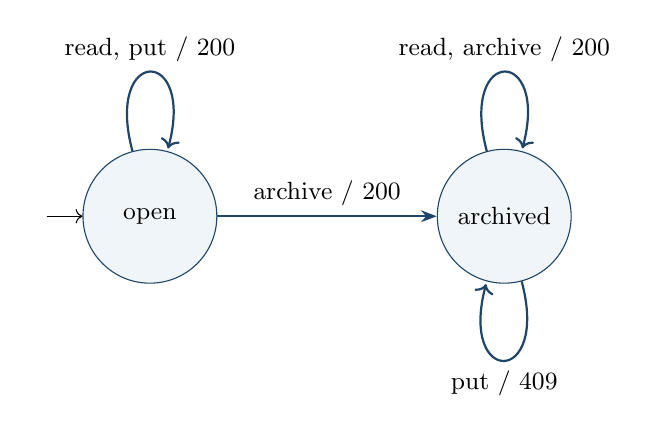
\begin{tikzpicture}[every state/.style={draw=inkblue,fill=pale,font=\small,minimum size=17mm}]
\node[state,initial,initial text={}] (o) at (0,0) {open};
\node[state] (a) at (4.5,0) {archived};
\draw[arr] (o) edge[loop above] node[above,font=\small]{read, put / 200}(o);
\draw[arr] (o)--node[above,font=\small]{archive / 200}(a);
\draw[arr] (a) edge[loop above] node[above,font=\small]{read, archive / 200}(a);
\draw[arr] (a) edge[loop below] node[below,font=\small]{put / 409}(a);
\end{tikzpicture}
\caption{The checked document policy for $h=1$. Labels give input event and output status. The table interpreter preserves these transitions for every finite event sequence}\label{fig:policy}
\end{figure}

\section{Formal artifact and executable validation}\label{sec:checking}
The artifact separates four forms of evidence: mathematical arguments in this paper, scoped TLAPS lemmas, bounded TLC exploration, and recorded executions of a Python reference controller. None substitutes for the others. In particular, the full parameterized inductive invariant and the asynchronous-to-atomic action correspondence have not been discharged in TLAPS. The reference implementation has no general refinement proof.

\subsection{Formalization and proof status}
\texttt{specification/Core.tla} and \texttt{AsyncController.tla} formalize ranked prerequisites, exact observations, historical acceptance, episode counts, request history, suspension, contract/authority changes, and publication evidence. The finite value relation is deliberately abstract: a proposed value is valid when it equals the observed source value. It is not an execution of the case-study table validator. Structural matching, failed candidate normalization and cross-view joint constraints are not fully connected to this protocol formalization; they are exercised separately in the implementation scenarios.

\texttt{AtomicController.tla} gives independent Attempt, Accept, Fail, Edit and Publish actions. A complete abstraction map must erase transport history and evidence detail while preserving attempts, episodes, accepted values and publication revision. Supplying that checked map remains an open obligation for Theorem~\ref{thm:refinement}; finite agreement cannot establish it.

The scoped proof modules are \texttt{Budget} (initial, increment and stuttering bounds for an isolated counter), \texttt{ControllerSafety} (the admission guard implies current authorized valid commitment), \texttt{StructuralKernelProofs} (coverage, unique producers and reference range under explicit construction hypotheses), and \texttt{DocumentPolicyProofs} (extensional validator equivalence, archive absorption and the archived-put conflict). These results support individual proof steps. They do not establish preservation of the whole controller invariant, history counting across changing episodes, or the concrete Python interpreter's correctness. The central proof gate is explicitly incomplete in \texttt{proofs/proof-status.json}.

TLAPS build \texttt{5f5037f} runs with its bundled Z3 4.8.9 in a pinned Linux container. Clean proof runs use strict mode and erase fingerprints. The trusted path includes the proof manager, translation and SMT backend; these runs do not replay SMT results in Isabelle. The first proof-development run failed obligations that lacked explicit references to construction/type assumptions. Those failures and the revised runs are preserved separately; no assumption equal to the advertised safety conclusion was introduced.

\subsection{Finite protocol exploration}
The TLC matrix is predefined in \texttt{models/matrix.yaml}. Each configuration fixes the job set, ranked parent relation, two abstract source/context values, attempt cap and environmental-change bound. One worker and a 768 MB Java heap are used with an explicit per-run timeout. The generated-state count includes repeated successors; it is not a transition or execution-trace count. Terminal self-loops are explicit and deadlock detection stays enabled. Exact commands, limits, tool versions, source hashes, status and raw output are retained for each run.

% BEGIN GENERATED TLC RESULTS
\begin{table}[tbp]
\centering
\caption{Detailed bounded TLC baseline results. $J$: jobs; $k$: attempt cap; $m$: environmental-change cap; $S$: distinct states; $G$: generated states including duplicates. Seconds include JVM startup for one invocation.}\label{tab:exploration}
\footnotesize
\setlength{\tabcolsep}{3pt}
\renewcommand{\arraystretch}{1.13}
\begin{tabularx}{\linewidth}{@{}Xrrrrrrr@{}}\toprule
Configuration & $J$ & $k$ & $m$ & $S$ & $G$ & $G/S$ & s\\\midrule
One job, k=1 & 1 & 1 & 1 & 87 & 316 & 3.63 & 5.844\\
One job, k=2 & 1 & 2 & 1 & 227 & 1,061 & 4.67 & 4.705\\
Chain, k=1 & 2 & 1 & 1 & 292 & 1,307 & 4.48 & 5.054\\
Chain, frozen & 2 & 2 & 0 & 23 & 107 & 4.65 & 3.523\\
Fan-out, frozen & 3 & 1 & 0 & 20 & 95 & 4.75 & 4.018\\
Workflow, frozen & 4 & 1 & 0 & 14 & 63 & 4.50 & 3.891\\
Reversion & 1 & 1 & 2 & 1,028 & 4,430 & 4.31 & 4.049\\
Parallel delivery & 2 & 1 & 1 & 475 & 2,345 & 4.94 & 5.186\\
Chain, temporal & 2 & 2 & 0 & 23 & 107 & 4.65 & 5.253\\
\bottomrule\end{tabularx}
\end{table}
% END GENERATED TLC RESULTS

The frozen-input temporal configuration checks eventual terminal classification, which may include exhausted jobs and suspended descendants. It assumes weak fairness of aggregate dispatch and request settlement, and permits no further environmental changes. It is a finite-instance liveness check, not a mechanized proof of Theorem~\ref{thm:termination} for arbitrary workflows. The two-change configuration exercises lifecycle and observation reversion; the independent-job configuration allows reordered delivery.

Mutation runs are separate from baseline correctness runs. Removing both cancellation and commit-time rechecking admits dispatch, edit, obsolete commitment. Resetting an exhausted counter violates the history-counting invariant. Omitting contract or selected-context identity permits commitment under changed inputs. Other mutations admit suspended publication, revoked authority or an old checked revision. Removing either obsolete-response defense alone survives because the other remains. Identity-reuse and tentative-write model mutants remain outstanding; their corresponding reference-controller regressions do not replace that missing model evidence.

The original manuscript referred to two earlier Python explorers and historical state counts. Their sources and reports were absent from the supplied checkout, so those counts are not reproduced or presented as current evidence. New TLC results use different models and must not be compared numerically to those earlier counts.

\section{An executable document-service case study}\label{sec:case-study}
The newly specified study uses four ranked views per source document: requirements, architecture, implementation and verification. A fifth security-review view can be added during execution. Each view has one stable target and one generated JSON attribute per document. A requirements proposal lists stable clauses R01--R03 and the current Boolean archive policy. An architecture proposal declares create/read/update/archive/list and an identifier type. The implementation proposal is the restricted table of Section~\ref{sec:discharged}; verification records clause coverage and an identifier type. Security review records required operation-assessment coverage. These coverage fields are checked metadata, not evidence that an independent security analysis or executable test suite was performed.

R01 requires stable string document identities and valid target/reference construction. Architecture locally permits a typed string or integer choice, but downstream structural expressions require strings; this gives a concrete locally valid proposal whose whole transaction must be rejected. R02 specifies the exact finite lifecycle state/status relation. R03 requires complete view metadata and matching architecture/verification identifier types before publication. The declared create/list operations are interface metadata; their storage and payload behavior are not implemented or verified by the six-row table. End-user authentication, confidentiality and persistent storage remain outside the study.

\begin{table}[tb]
\caption{Ranked case-study binding contracts}\label{tab:bindings}
\small\begin{tabularx}{\linewidth}{@{}lXX@{}}\toprule
View & Declared inputs & Local check\\\midrule
Requirements & Source policy & Clause IDs, exact Boolean policy\\
Architecture & Usable requirements & Operation list, typed ID choice\\
Implementation & Interface, source clause, selected findings & Exact six-row policy table\\
Verification & Table, source clause, selected findings & Coverage and typed ID metadata\\
Security (added) & Verification, selected findings & Operation-assessment coverage\\\bottomrule
\end{tabularx}
\end{table}

The controller serializes public actions with one in-process lock. It copies a candidate, installs the proposed primitive value privately, and recomputes complete downstream structure before installing any effect. Request identities and counters survive all changes within one controller lifetime, but are not durable across restart. Source/context ingress is a trusted-host capability; workers receive no direct edit authority. Proposal providers are deterministic scripts, with no model credentials or remote calls.

Observations store exact canonical JSON, including the owner, contract, source clause, usable predecessor values and full selected finding membership. Audit-only context versions are excluded from worker inputs. Historical accepted records can be reused after reactivation only under equal observation, compatible owner/contract and current permission. Regranting the same owner under an unchanged contract permits such reuse; policies forbidding it must change contract identity. These choices implement the intended A0--A4 disciplines within the documented in-process trust boundary; they do not mechanically discharge every abstract interface obligation. A5--A6 govern scheduling; A7 is discharged only for the exact finite policy relation, with weaker metadata guarantees for the other validators.

Figure~\ref{fig:case-trace} shows a representative pending-request edit. A source reversion does not restore authority to the canceled request, even when the observation bytes return to their earlier value. A separate scenario changes the architecture contract, repairs it to equal output, and restores compatible descendants from cache without another downstream request.
\begin{figure}[tb]
\centering
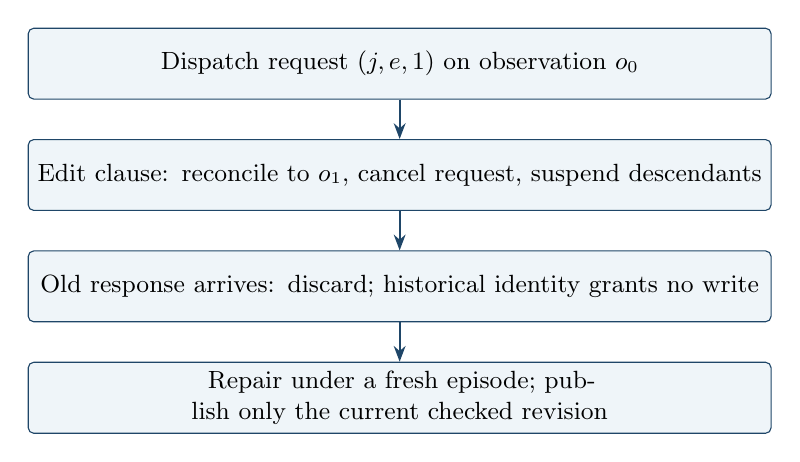
\begin{tikzpicture}[node distance=5mm, every node/.style={font=\small}]
\node[box,text width=92mm] (a) {Dispatch request $(j,e,1)$ on observation $o_0$};
\node[box,text width=92mm,below=of a] (b) {Edit clause: reconcile to $o_1$, cancel request, suspend descendants};
\node[box,text width=92mm,below=of b] (c) {Old response arrives: discard; historical identity grants no write};
\node[box,text width=92mm,below=of c] (d) {Repair under a fresh episode; publish only the current checked revision};
\draw[arr] (a)--(b); \draw[arr] (b)--(c); \draw[arr] (c)--(d);
\end{tikzpicture}
\caption{A scripted change trace through atomic controller actions. The final publication is conditional on all local and joint obligations}\label{fig:case-trace}
\end{figure}

Scenario inputs and independent expectations are fixed in \texttt{case-study/document-service/scenarios/campaign.json}. They cover unchanged/unselected content, selector additions, pending edits, source reversion, timeout/duplicate delivery, exhaustion, suspension/cache restoration, joint conflict, failed candidate rollback, reviewer changes, authority/contract changes, same-version context writers, stale global checks, observer loss and malformed ingress. The finite-language campaign separately exhausts typed tables and bounded event words; malformed table cases include absent/duplicate rows and incorrect primitive types.

% BEGIN GENERATED CAMPAIGN SUMMARY
The scripted campaign passed 28 of 28 predefined scenarios. The separate checker admitted 28 of 28 recorded traces and rejected 9 deliberately corrupted traces. The policy-language campaign enumerated 8,192 typed tables across both policy settings, and exercised all 1,093 event words of length at most six for the strict table. The separate nonvacuity campaign produced 5 expected shortest reachability witnesses. The scoped TLAPS run discharged 25 generated obligations across the reported lemma modules; this count includes supporting obligations and does not discharge the central controller invariant or refinement theorem.
% END GENERATED CAMPAIGN SUMMARY

The trace checker is implemented separately from controller admission code and independently evaluates finite contracts. It checks state continuity, ranked availability, exact observations, dispatch identity/counters, historical provenance, current authority, rejection rollback and publication snapshots. It independently reconstructs deterministic reconciliation effects, but its recorded events are trusted; it cannot detect a silently omitted final trace suffix without an external completion marker. Thus these are conformance results for recorded executions, not a general implementation-refinement theorem. Deterministic scenarios are neither independent statistical samples nor measurements of language-model quality or speed.

Reproduction commands, raw manifests, failed proof attempts and generated table-cell provenance are supplied locally. \texttt{python scripts/reproduce.py all --profile core} runs each stage and deliberately returns failure while baseline evidence or central proof obligations remain incomplete. A successful scenario or scoped lemma run cannot hide those open gates.

% BEGIN GENERATED DETAILED RESULTS
\section{Experimental results and discussion}\label{sec:results}

\subsection{Evidence selection and interpretation}

The following descriptive analysis covers the final archived campaign of each experiment type, together with failed proof-development trials and clean-directory reproductions. Every plotted value is derived from immutable reports, trace records or shortest-path logs; the input hashes and derived cells are recorded in \texttt{results/processed/document-service-v1/detailed-results.json}. Repeated development runs remain in the archive inventory. They are reproducibility/debugging records, not independent samples. No confidence interval, significance test, generative success probability or measured speedup is inferred from these deterministic fixtures and exhaustive finite enumerations.

\subsection{State-space structure and model-checking effort}

\begin{figure}[tbp]
\centering
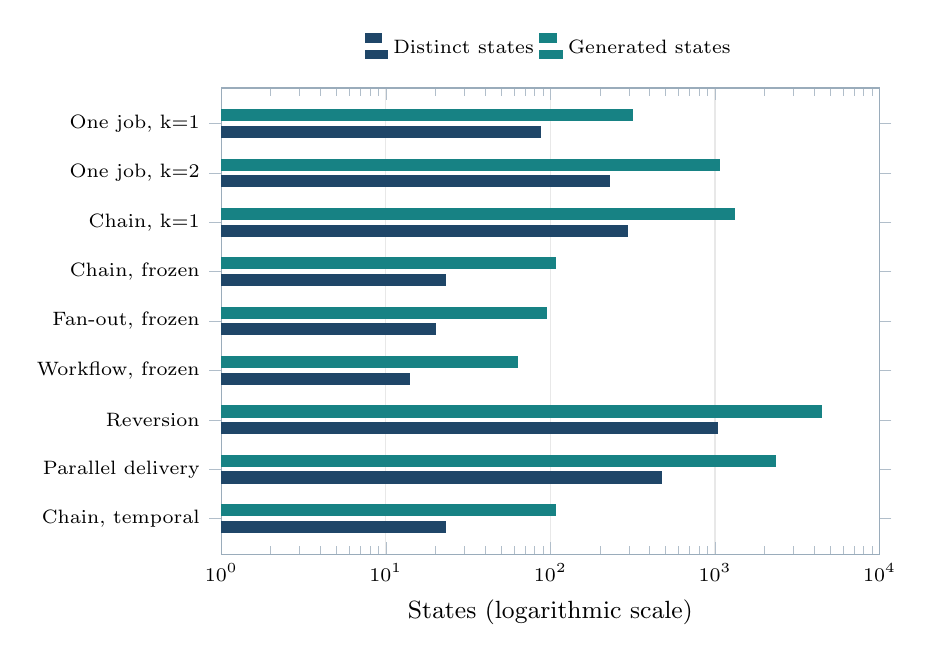
\begin{tikzpicture}
\begin{axis}[vgcplot,xbar,bar width=4pt,width=.82\linewidth,height=7.5cm,
 xmode=log,log basis x=10,xmin=1,xmax=10000,
 xlabel={States (logarithmic scale)},ylabel={},
 ytick={0,1,2,3,4,5,6,7,8},yticklabels={{One job, k=1},{One job, k=2},{Chain, k=1},{Chain, frozen},{Fan-out, frozen},{Workflow, frozen},{Reversion},{Parallel delivery},{Chain, temporal}},
 y dir=reverse,enlarge y limits=.09,
 legend style={at={(.5,1.04)},anchor=south,legend columns=2,draw=none}]
\addplot[fill=inkblue,draw=inkblue] coordinates {(87,0) (227,1) (292,2) (23,3) (20,4) (14,5) (1028,6) (475,7) (23,8)};
\addplot[fill=resultteal,draw=resultteal] coordinates {(316,0) (1061,1) (1307,2) (107,3) (95,4) (63,5) (4430,6) (2345,7) (107,8)};
\legend{Distinct states,Generated states}
\end{axis}
\end{tikzpicture}
\caption{State-space profiles for the nine baseline configurations. The log axis makes frozen and changing-input instances legible together. Generated states include repeated successors; the gap is not a count of independent tests or proof strength.}\label{fig:state-space}
\end{figure}

Figure~\ref{fig:state-space} and Table~\ref{tab:exploration} expose the effect of the declared bounds. Raising the one-job attempt cap from one to two increases distinct states from 87 to 227 (2.61 times), while permitting two environmental changes in the reversion instance reaches 1,028 distinct states. These are separate configurations, not asymptotic scaling estimates. The frozen four-stage workflow has only 14 distinct states: strict prerequisites serialize eligibility and the environment cannot edit it. A small count here reflects restricted behavior, not stronger verification or superior runtime performance.

The $G/S$ ratio in Table~\ref{tab:exploration} describes repeated generated successors relative to distinct states. It is not a cache-hit rate of the Python controller. The recorded wall times are single local invocations with JVM startup, fixed one-worker execution and a 768 MB heap. Startup and host activity can dominate such small models; these durations document completed runs within their time limits and are not a controlled throughput comparison. The temporal configuration uses explicit aggregate fairness and frozen inputs; its passing result remains a finite liveness check.

\subsection{Proof obligations, failed trials and remaining scope}

\begin{table}[tbp]
\centering
\caption{Scoped TLAPS outcomes for the final clean run. Counts are generated obligations, including supporting obligations; these are not counts of full controller theorems.}\label{tab:proof-results}
\footnotesize
\setlength{\tabcolsep}{3pt}
\renewcommand{\arraystretch}{1.13}
\begin{tabularx}{\linewidth}{@{}Xrrrrl@{}}\toprule
Module & Total & Proved & Omitted & s & Status\\\midrule
Budget & 8 & 8 & 0 & 6.008 & Passed\\
ControllerSafety & 2 & 2 & 0 & 4.765 & Passed\\
StructuralKernelProofs & 9 & 9 & 0 & 4.555 & Passed\\
DocumentPolicyProofs & 6 & 6 & 0 & 4.116 & Passed\\
\bottomrule\end{tabularx}
\end{table}

\begin{table}[tbp]
\centering
\caption{Recorded initial proof-development trial. A failed obligation is preserved as a failed proof attempt, not a reachable-state counterexample. Later explicit type/construction-assumption references repaired these scoped proofs.}\label{tab:proof-development}
\footnotesize
\setlength{\tabcolsep}{3pt}
\renewcommand{\arraystretch}{1.13}
\begin{tabularx}{\linewidth}{@{}Xrrrl@{}}\toprule
Module & Total & Failed & s & Status\\\midrule
Budget & 7 & 1 & 8.334 & Failed\\
ControllerSafety & 2 & 0 & 5.260 & Passed\\
StructuralKernelProofs & 6 & 2 & 7.491 & Failed\\
DocumentPolicyProofs & 6 & 0 & 2.491 & Passed\\
\bottomrule\end{tabularx}
\end{table}

Table~\ref{tab:proof-results} separates the successful scoped modules from the unfinished central proof gate. The isolated counter lemma does not count arbitrary controller histories; the admission lemma derives its conclusion from the explicit commit guard, not from an induction over all actions. Kernel results rely on injective constructors and current reference domains, while policy results concern the restricted extensional relation. Table~\ref{tab:proof-development} retains the earlier failures, including missing explicit assumption references. The increase in generated obligations after repair reflects proof elaboration and cited assumptions, not additional independently verified software features. Internal review also exposed insufficient history-shape constraints in a proposed induction invariant; strengthening those constraints excludes that review witness but does not establish the full invariant's inductiveness.

\subsection{Mutation sensitivity and nonvacuity}

\begin{figure}[tbp]\centering
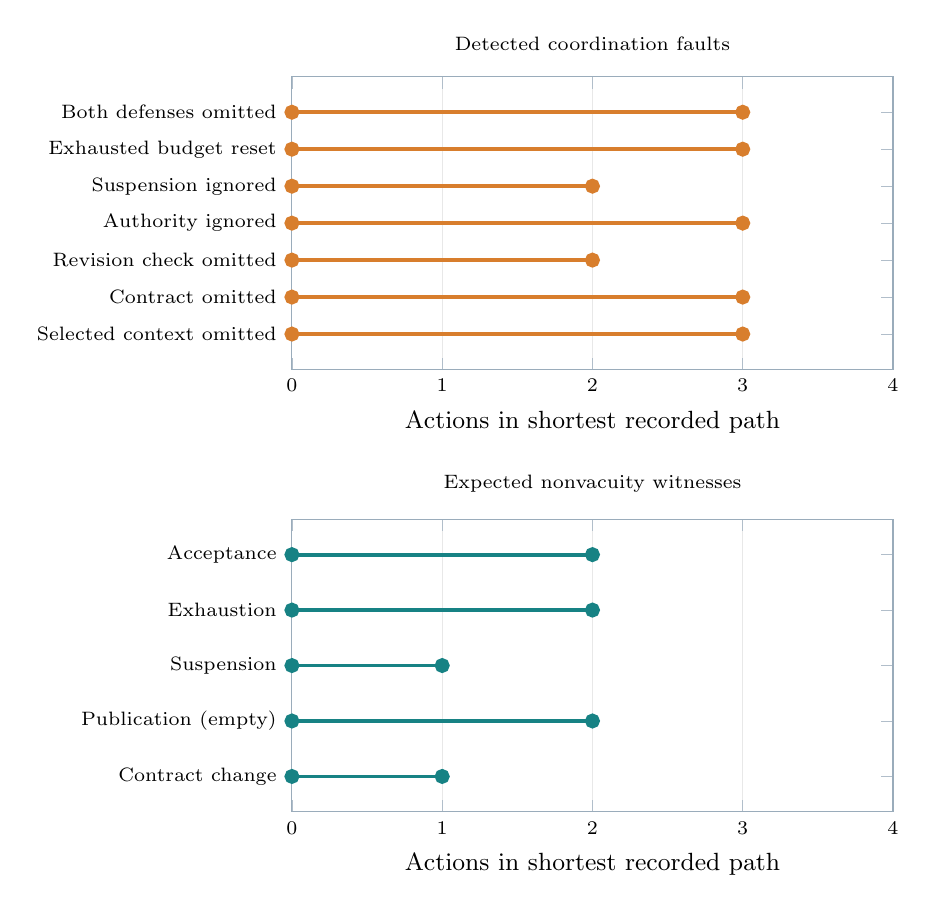
\begin{tikzpicture}
\begin{groupplot}[group style={group size=1 by 2,vertical sep=1.9cm},vgcplot,width=.76\linewidth,height=5.3cm,xmin=0,xmax=4,xtick={0,1,2,3,4},yticklabel style={xshift=-2pt},y dir=reverse,enlarge y limits=.16]
\nextgroupplot[title={Detected coordination faults},xlabel={Actions in shortest recorded path},ytick={0,1,2,3,4,5,6},yticklabels={{Both defenses omitted},{Exhausted budget reset},{Suspension ignored},{Authority ignored},{Revision check omitted},{Contract omitted},{Selected context omitted}}]
\addplot[resultamber,line width=1.4pt,mark=*,mark options={fill=resultamber}] coordinates {(0,0) (3,0)};
\addplot[resultamber,line width=1.4pt,mark=*,mark options={fill=resultamber}] coordinates {(0,1) (3,1)};
\addplot[resultamber,line width=1.4pt,mark=*,mark options={fill=resultamber}] coordinates {(0,2) (2,2)};
\addplot[resultamber,line width=1.4pt,mark=*,mark options={fill=resultamber}] coordinates {(0,3) (3,3)};
\addplot[resultamber,line width=1.4pt,mark=*,mark options={fill=resultamber}] coordinates {(0,4) (2,4)};
\addplot[resultamber,line width=1.4pt,mark=*,mark options={fill=resultamber}] coordinates {(0,5) (3,5)};
\addplot[resultamber,line width=1.4pt,mark=*,mark options={fill=resultamber}] coordinates {(0,6) (3,6)};
\nextgroupplot[title={Expected nonvacuity witnesses},xlabel={Actions in shortest recorded path},ytick={0,1,2,3,4},yticklabels={{Acceptance},{Exhaustion},{Suspension},{Publication (empty)},{Contract change}}]
\addplot[resultteal,line width=1.4pt,mark=*,mark options={fill=resultteal}] coordinates {(0,0) (2,0)};
\addplot[resultteal,line width=1.4pt,mark=*,mark options={fill=resultteal}] coordinates {(0,1) (2,1)};
\addplot[resultteal,line width=1.4pt,mark=*,mark options={fill=resultteal}] coordinates {(0,2) (1,2)};
\addplot[resultteal,line width=1.4pt,mark=*,mark options={fill=resultteal}] coordinates {(0,3) (2,3)};
\addplot[resultteal,line width=1.4pt,mark=*,mark options={fill=resultteal}] coordinates {(0,4) (1,4)};
\end{groupplot}\end{tikzpicture}
\caption{Shortest paths extracted from TLC counterexample logs, excluding the initial state. The upper panel records actual safety violations in deliberate mutants; the lower panel records desired reachable states by violating their negations. The two surviving single-defense mutants have no counterexample path and are excluded from the upper panel, not assigned length zero.}\label{fig:shortest-paths}
\end{figure}

\begin{table}[tbp]
\centering
\caption{Complete mutant campaign. CEX: intended property violated; survive: exhaustive pass under the remaining defense. Path length excludes the initial state; -- means no counterexample was found. $S$: distinct states; $G$: generated states. All use one job, k=1 and at most one environmental change.}\label{tab:mutation-detail}
\scriptsize
\setlength{\tabcolsep}{3pt}
\renewcommand{\arraystretch}{1.13}
\begin{tabularx}{\linewidth}{@{}Xlrrrrl@{}}\toprule
Fault & Target & Path & $S$ & $G$ & s & Result\\\midrule
Cancellation omitted & Safety invariant & -- & 93 & 328 & 4.763 & Survive\\
Recheck omitted & Safety invariant & -- & 87 & 358 & 4.741 & Survive\\
Both defenses omitted & Current observation & 3 & 31 & 69 & 5.012 & CEX\\
Exhausted budget reset & Episode accounting & 3 & 45 & 89 & 5.526 & CEX\\
Suspension ignored & No suspended stage & 2 & 14 & 20 & 3.524 & CEX\\
Authority ignored & Current authority & 3 & 32 & 98 & 5.218 & CEX\\
Revision check omitted & Checked revision & 2 & 14 & 21 & 4.108 & CEX\\
Contract omitted & Contract identity & 3 & 33 & 60 & 4.134 & CEX\\
Selected context omitted & Context identity & 3 & 32 & 57 & 4.926 & CEX\\
\bottomrule\end{tabularx}
\end{table}

\begin{table}[tbp]
\centering
\caption{Nonvacuity campaign: shortest desired-state witnesses. Each expected counterexample violates the negation of a reachability target and therefore indicates coverage, not an error in the baseline protocol.}\label{tab:witness-detail}
\footnotesize
\setlength{\tabcolsep}{3pt}
\renewcommand{\arraystretch}{1.13}
\begin{tabularx}{\linewidth}{@{}Xrrrr@{}}\toprule
Reachability target & Actions & Distinct & Generated & s\\\midrule
Acceptance & 2 & 21 & 32 & 4.890\\
Exhaustion & 2 & 22 & 33 & 5.526\\
Suspension & 1 & 6 & 7 & 5.227\\
Publication (empty) & 2 & 14 & 21 & 4.560\\
Contract change & 1 & 5 & 6 & 4.617\\
\bottomrule\end{tabularx}
\end{table}

Figure~\ref{fig:shortest-paths} makes the short failure mechanisms visible: obsolete commitment, counter reset and changed contract/context require only a few actions in these abstractions. The two surviving mutants remove one obsolete-response defense at a time. Their survival is expected redundancy under the other defense, not evidence that the omitted guard is unnecessary in a larger runtime. A mutation is counted as detected only when its named intended property fails. Exploration stops at the first shortest counterexample, so mutant state counts cannot be compared to exhaustive baseline state counts as a measure of scalability. Table~\ref{tab:witness-detail} independently demonstrates reachable acceptance, exhaustion, suspension, publication and contract change; a safety invariant could otherwise pass in a model that never admits useful work.

The shortest publication witness first deletes the only job and then publishes the permitted zero-match workflow. It therefore establishes reachability of publication but does not itself demonstrate publication after nonempty generated work. S01, S20 and S26 supply recorded implementation executions with successful nonempty publication; a separate shortest formal witness requiring a nonempty accepted workflow has not been collected here. Keeping this distinction visible prevents a reachable empty completion from being mistaken for coverage of every successful workflow.

\subsection{Scenario-level workload and terminal outcomes}

\begin{figure}[tbp]\centering
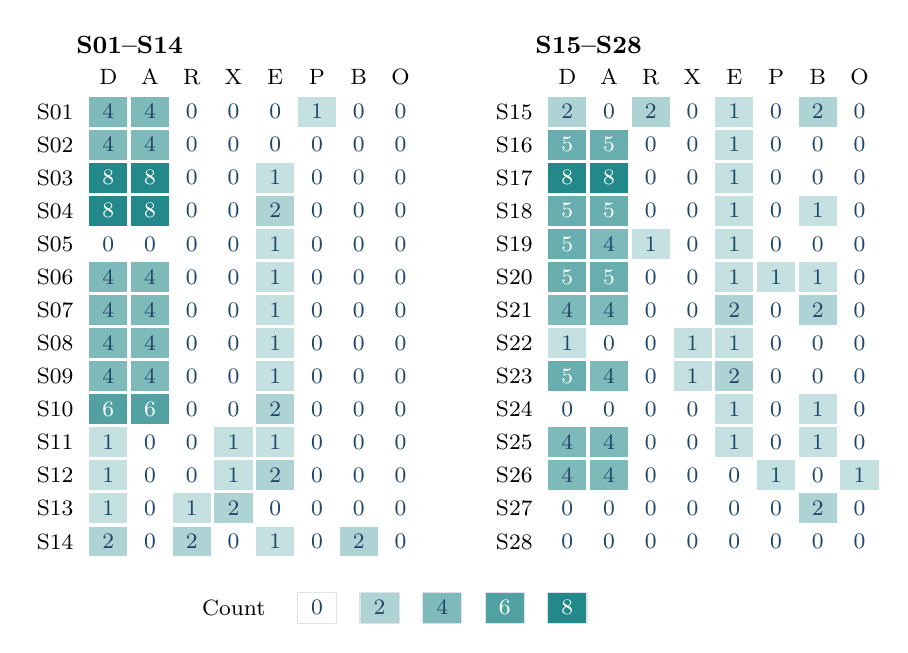
\begin{tikzpicture}[x=.53cm,y=.42cm,every node/.style={font=\footnotesize}]
\node[anchor=west,font=\small\bfseries] at (-1,2.0) {S01--S14};
\node at (0,1.05) {D};
\node at (1,1.05) {A};
\node at (2,1.05) {R};
\node at (3,1.05) {X};
\node at (4,1.05) {E};
\node at (5,1.05) {P};
\node at (6,1.05) {B};
\node at (7,1.05) {O};
\node[anchor=east] at (-0.6,0) {S01};
\filldraw[fill=resultteal!55!white,draw=white] (-0.47,-0.47) rectangle ++(.94,.94);
\node[text=inkblue] at (0,0) {4};
\filldraw[fill=resultteal!55!white,draw=white] (0.53,-0.47) rectangle ++(.94,.94);
\node[text=inkblue] at (1,0) {4};
\filldraw[fill=resultteal!0!white,draw=white] (1.53,-0.47) rectangle ++(.94,.94);
\node[text=inkblue] at (2,0) {0};
\filldraw[fill=resultteal!0!white,draw=white] (2.5300000000000002,-0.47) rectangle ++(.94,.94);
\node[text=inkblue] at (3,0) {0};
\filldraw[fill=resultteal!0!white,draw=white] (3.5300000000000002,-0.47) rectangle ++(.94,.94);
\node[text=inkblue] at (4,0) {0};
\filldraw[fill=resultteal!25!white,draw=white] (4.53,-0.47) rectangle ++(.94,.94);
\node[text=inkblue] at (5,0) {1};
\filldraw[fill=resultteal!0!white,draw=white] (5.53,-0.47) rectangle ++(.94,.94);
\node[text=inkblue] at (6,0) {0};
\filldraw[fill=resultteal!0!white,draw=white] (6.53,-0.47) rectangle ++(.94,.94);
\node[text=inkblue] at (7,0) {0};
\node[anchor=east] at (-0.6,-1) {S02};
\filldraw[fill=resultteal!55!white,draw=white] (-0.47,-1.47) rectangle ++(.94,.94);
\node[text=inkblue] at (0,-1) {4};
\filldraw[fill=resultteal!55!white,draw=white] (0.53,-1.47) rectangle ++(.94,.94);
\node[text=inkblue] at (1,-1) {4};
\filldraw[fill=resultteal!0!white,draw=white] (1.53,-1.47) rectangle ++(.94,.94);
\node[text=inkblue] at (2,-1) {0};
\filldraw[fill=resultteal!0!white,draw=white] (2.5300000000000002,-1.47) rectangle ++(.94,.94);
\node[text=inkblue] at (3,-1) {0};
\filldraw[fill=resultteal!0!white,draw=white] (3.5300000000000002,-1.47) rectangle ++(.94,.94);
\node[text=inkblue] at (4,-1) {0};
\filldraw[fill=resultteal!0!white,draw=white] (4.53,-1.47) rectangle ++(.94,.94);
\node[text=inkblue] at (5,-1) {0};
\filldraw[fill=resultteal!0!white,draw=white] (5.53,-1.47) rectangle ++(.94,.94);
\node[text=inkblue] at (6,-1) {0};
\filldraw[fill=resultteal!0!white,draw=white] (6.53,-1.47) rectangle ++(.94,.94);
\node[text=inkblue] at (7,-1) {0};
\node[anchor=east] at (-0.6,-2) {S03};
\filldraw[fill=resultteal!95!white,draw=white] (-0.47,-2.4699999999999998) rectangle ++(.94,.94);
\node[text=white] at (0,-2) {8};
\filldraw[fill=resultteal!95!white,draw=white] (0.53,-2.4699999999999998) rectangle ++(.94,.94);
\node[text=white] at (1,-2) {8};
\filldraw[fill=resultteal!0!white,draw=white] (1.53,-2.4699999999999998) rectangle ++(.94,.94);
\node[text=inkblue] at (2,-2) {0};
\filldraw[fill=resultteal!0!white,draw=white] (2.5300000000000002,-2.4699999999999998) rectangle ++(.94,.94);
\node[text=inkblue] at (3,-2) {0};
\filldraw[fill=resultteal!25!white,draw=white] (3.5300000000000002,-2.4699999999999998) rectangle ++(.94,.94);
\node[text=inkblue] at (4,-2) {1};
\filldraw[fill=resultteal!0!white,draw=white] (4.53,-2.4699999999999998) rectangle ++(.94,.94);
\node[text=inkblue] at (5,-2) {0};
\filldraw[fill=resultteal!0!white,draw=white] (5.53,-2.4699999999999998) rectangle ++(.94,.94);
\node[text=inkblue] at (6,-2) {0};
\filldraw[fill=resultteal!0!white,draw=white] (6.53,-2.4699999999999998) rectangle ++(.94,.94);
\node[text=inkblue] at (7,-2) {0};
\node[anchor=east] at (-0.6,-3) {S04};
\filldraw[fill=resultteal!95!white,draw=white] (-0.47,-3.4699999999999998) rectangle ++(.94,.94);
\node[text=white] at (0,-3) {8};
\filldraw[fill=resultteal!95!white,draw=white] (0.53,-3.4699999999999998) rectangle ++(.94,.94);
\node[text=white] at (1,-3) {8};
\filldraw[fill=resultteal!0!white,draw=white] (1.53,-3.4699999999999998) rectangle ++(.94,.94);
\node[text=inkblue] at (2,-3) {0};
\filldraw[fill=resultteal!0!white,draw=white] (2.5300000000000002,-3.4699999999999998) rectangle ++(.94,.94);
\node[text=inkblue] at (3,-3) {0};
\filldraw[fill=resultteal!35!white,draw=white] (3.5300000000000002,-3.4699999999999998) rectangle ++(.94,.94);
\node[text=inkblue] at (4,-3) {2};
\filldraw[fill=resultteal!0!white,draw=white] (4.53,-3.4699999999999998) rectangle ++(.94,.94);
\node[text=inkblue] at (5,-3) {0};
\filldraw[fill=resultteal!0!white,draw=white] (5.53,-3.4699999999999998) rectangle ++(.94,.94);
\node[text=inkblue] at (6,-3) {0};
\filldraw[fill=resultteal!0!white,draw=white] (6.53,-3.4699999999999998) rectangle ++(.94,.94);
\node[text=inkblue] at (7,-3) {0};
\node[anchor=east] at (-0.6,-4) {S05};
\filldraw[fill=resultteal!0!white,draw=white] (-0.47,-4.47) rectangle ++(.94,.94);
\node[text=inkblue] at (0,-4) {0};
\filldraw[fill=resultteal!0!white,draw=white] (0.53,-4.47) rectangle ++(.94,.94);
\node[text=inkblue] at (1,-4) {0};
\filldraw[fill=resultteal!0!white,draw=white] (1.53,-4.47) rectangle ++(.94,.94);
\node[text=inkblue] at (2,-4) {0};
\filldraw[fill=resultteal!0!white,draw=white] (2.5300000000000002,-4.47) rectangle ++(.94,.94);
\node[text=inkblue] at (3,-4) {0};
\filldraw[fill=resultteal!25!white,draw=white] (3.5300000000000002,-4.47) rectangle ++(.94,.94);
\node[text=inkblue] at (4,-4) {1};
\filldraw[fill=resultteal!0!white,draw=white] (4.53,-4.47) rectangle ++(.94,.94);
\node[text=inkblue] at (5,-4) {0};
\filldraw[fill=resultteal!0!white,draw=white] (5.53,-4.47) rectangle ++(.94,.94);
\node[text=inkblue] at (6,-4) {0};
\filldraw[fill=resultteal!0!white,draw=white] (6.53,-4.47) rectangle ++(.94,.94);
\node[text=inkblue] at (7,-4) {0};
\node[anchor=east] at (-0.6,-5) {S06};
\filldraw[fill=resultteal!55!white,draw=white] (-0.47,-5.47) rectangle ++(.94,.94);
\node[text=inkblue] at (0,-5) {4};
\filldraw[fill=resultteal!55!white,draw=white] (0.53,-5.47) rectangle ++(.94,.94);
\node[text=inkblue] at (1,-5) {4};
\filldraw[fill=resultteal!0!white,draw=white] (1.53,-5.47) rectangle ++(.94,.94);
\node[text=inkblue] at (2,-5) {0};
\filldraw[fill=resultteal!0!white,draw=white] (2.5300000000000002,-5.47) rectangle ++(.94,.94);
\node[text=inkblue] at (3,-5) {0};
\filldraw[fill=resultteal!25!white,draw=white] (3.5300000000000002,-5.47) rectangle ++(.94,.94);
\node[text=inkblue] at (4,-5) {1};
\filldraw[fill=resultteal!0!white,draw=white] (4.53,-5.47) rectangle ++(.94,.94);
\node[text=inkblue] at (5,-5) {0};
\filldraw[fill=resultteal!0!white,draw=white] (5.53,-5.47) rectangle ++(.94,.94);
\node[text=inkblue] at (6,-5) {0};
\filldraw[fill=resultteal!0!white,draw=white] (6.53,-5.47) rectangle ++(.94,.94);
\node[text=inkblue] at (7,-5) {0};
\node[anchor=east] at (-0.6,-6) {S07};
\filldraw[fill=resultteal!55!white,draw=white] (-0.47,-6.47) rectangle ++(.94,.94);
\node[text=inkblue] at (0,-6) {4};
\filldraw[fill=resultteal!55!white,draw=white] (0.53,-6.47) rectangle ++(.94,.94);
\node[text=inkblue] at (1,-6) {4};
\filldraw[fill=resultteal!0!white,draw=white] (1.53,-6.47) rectangle ++(.94,.94);
\node[text=inkblue] at (2,-6) {0};
\filldraw[fill=resultteal!0!white,draw=white] (2.5300000000000002,-6.47) rectangle ++(.94,.94);
\node[text=inkblue] at (3,-6) {0};
\filldraw[fill=resultteal!25!white,draw=white] (3.5300000000000002,-6.47) rectangle ++(.94,.94);
\node[text=inkblue] at (4,-6) {1};
\filldraw[fill=resultteal!0!white,draw=white] (4.53,-6.47) rectangle ++(.94,.94);
\node[text=inkblue] at (5,-6) {0};
\filldraw[fill=resultteal!0!white,draw=white] (5.53,-6.47) rectangle ++(.94,.94);
\node[text=inkblue] at (6,-6) {0};
\filldraw[fill=resultteal!0!white,draw=white] (6.53,-6.47) rectangle ++(.94,.94);
\node[text=inkblue] at (7,-6) {0};
\node[anchor=east] at (-0.6,-7) {S08};
\filldraw[fill=resultteal!55!white,draw=white] (-0.47,-7.47) rectangle ++(.94,.94);
\node[text=inkblue] at (0,-7) {4};
\filldraw[fill=resultteal!55!white,draw=white] (0.53,-7.47) rectangle ++(.94,.94);
\node[text=inkblue] at (1,-7) {4};
\filldraw[fill=resultteal!0!white,draw=white] (1.53,-7.47) rectangle ++(.94,.94);
\node[text=inkblue] at (2,-7) {0};
\filldraw[fill=resultteal!0!white,draw=white] (2.5300000000000002,-7.47) rectangle ++(.94,.94);
\node[text=inkblue] at (3,-7) {0};
\filldraw[fill=resultteal!25!white,draw=white] (3.5300000000000002,-7.47) rectangle ++(.94,.94);
\node[text=inkblue] at (4,-7) {1};
\filldraw[fill=resultteal!0!white,draw=white] (4.53,-7.47) rectangle ++(.94,.94);
\node[text=inkblue] at (5,-7) {0};
\filldraw[fill=resultteal!0!white,draw=white] (5.53,-7.47) rectangle ++(.94,.94);
\node[text=inkblue] at (6,-7) {0};
\filldraw[fill=resultteal!0!white,draw=white] (6.53,-7.47) rectangle ++(.94,.94);
\node[text=inkblue] at (7,-7) {0};
\node[anchor=east] at (-0.6,-8) {S09};
\filldraw[fill=resultteal!55!white,draw=white] (-0.47,-8.47) rectangle ++(.94,.94);
\node[text=inkblue] at (0,-8) {4};
\filldraw[fill=resultteal!55!white,draw=white] (0.53,-8.47) rectangle ++(.94,.94);
\node[text=inkblue] at (1,-8) {4};
\filldraw[fill=resultteal!0!white,draw=white] (1.53,-8.47) rectangle ++(.94,.94);
\node[text=inkblue] at (2,-8) {0};
\filldraw[fill=resultteal!0!white,draw=white] (2.5300000000000002,-8.47) rectangle ++(.94,.94);
\node[text=inkblue] at (3,-8) {0};
\filldraw[fill=resultteal!25!white,draw=white] (3.5300000000000002,-8.47) rectangle ++(.94,.94);
\node[text=inkblue] at (4,-8) {1};
\filldraw[fill=resultteal!0!white,draw=white] (4.53,-8.47) rectangle ++(.94,.94);
\node[text=inkblue] at (5,-8) {0};
\filldraw[fill=resultteal!0!white,draw=white] (5.53,-8.47) rectangle ++(.94,.94);
\node[text=inkblue] at (6,-8) {0};
\filldraw[fill=resultteal!0!white,draw=white] (6.53,-8.47) rectangle ++(.94,.94);
\node[text=inkblue] at (7,-8) {0};
\node[anchor=east] at (-0.6,-9) {S10};
\filldraw[fill=resultteal!75!white,draw=white] (-0.47,-9.47) rectangle ++(.94,.94);
\node[text=white] at (0,-9) {6};
\filldraw[fill=resultteal!75!white,draw=white] (0.53,-9.47) rectangle ++(.94,.94);
\node[text=white] at (1,-9) {6};
\filldraw[fill=resultteal!0!white,draw=white] (1.53,-9.47) rectangle ++(.94,.94);
\node[text=inkblue] at (2,-9) {0};
\filldraw[fill=resultteal!0!white,draw=white] (2.5300000000000002,-9.47) rectangle ++(.94,.94);
\node[text=inkblue] at (3,-9) {0};
\filldraw[fill=resultteal!35!white,draw=white] (3.5300000000000002,-9.47) rectangle ++(.94,.94);
\node[text=inkblue] at (4,-9) {2};
\filldraw[fill=resultteal!0!white,draw=white] (4.53,-9.47) rectangle ++(.94,.94);
\node[text=inkblue] at (5,-9) {0};
\filldraw[fill=resultteal!0!white,draw=white] (5.53,-9.47) rectangle ++(.94,.94);
\node[text=inkblue] at (6,-9) {0};
\filldraw[fill=resultteal!0!white,draw=white] (6.53,-9.47) rectangle ++(.94,.94);
\node[text=inkblue] at (7,-9) {0};
\node[anchor=east] at (-0.6,-10) {S11};
\filldraw[fill=resultteal!25!white,draw=white] (-0.47,-10.47) rectangle ++(.94,.94);
\node[text=inkblue] at (0,-10) {1};
\filldraw[fill=resultteal!0!white,draw=white] (0.53,-10.47) rectangle ++(.94,.94);
\node[text=inkblue] at (1,-10) {0};
\filldraw[fill=resultteal!0!white,draw=white] (1.53,-10.47) rectangle ++(.94,.94);
\node[text=inkblue] at (2,-10) {0};
\filldraw[fill=resultteal!25!white,draw=white] (2.5300000000000002,-10.47) rectangle ++(.94,.94);
\node[text=inkblue] at (3,-10) {1};
\filldraw[fill=resultteal!25!white,draw=white] (3.5300000000000002,-10.47) rectangle ++(.94,.94);
\node[text=inkblue] at (4,-10) {1};
\filldraw[fill=resultteal!0!white,draw=white] (4.53,-10.47) rectangle ++(.94,.94);
\node[text=inkblue] at (5,-10) {0};
\filldraw[fill=resultteal!0!white,draw=white] (5.53,-10.47) rectangle ++(.94,.94);
\node[text=inkblue] at (6,-10) {0};
\filldraw[fill=resultteal!0!white,draw=white] (6.53,-10.47) rectangle ++(.94,.94);
\node[text=inkblue] at (7,-10) {0};
\node[anchor=east] at (-0.6,-11) {S12};
\filldraw[fill=resultteal!25!white,draw=white] (-0.47,-11.47) rectangle ++(.94,.94);
\node[text=inkblue] at (0,-11) {1};
\filldraw[fill=resultteal!0!white,draw=white] (0.53,-11.47) rectangle ++(.94,.94);
\node[text=inkblue] at (1,-11) {0};
\filldraw[fill=resultteal!0!white,draw=white] (1.53,-11.47) rectangle ++(.94,.94);
\node[text=inkblue] at (2,-11) {0};
\filldraw[fill=resultteal!25!white,draw=white] (2.5300000000000002,-11.47) rectangle ++(.94,.94);
\node[text=inkblue] at (3,-11) {1};
\filldraw[fill=resultteal!35!white,draw=white] (3.5300000000000002,-11.47) rectangle ++(.94,.94);
\node[text=inkblue] at (4,-11) {2};
\filldraw[fill=resultteal!0!white,draw=white] (4.53,-11.47) rectangle ++(.94,.94);
\node[text=inkblue] at (5,-11) {0};
\filldraw[fill=resultteal!0!white,draw=white] (5.53,-11.47) rectangle ++(.94,.94);
\node[text=inkblue] at (6,-11) {0};
\filldraw[fill=resultteal!0!white,draw=white] (6.53,-11.47) rectangle ++(.94,.94);
\node[text=inkblue] at (7,-11) {0};
\node[anchor=east] at (-0.6,-12) {S13};
\filldraw[fill=resultteal!25!white,draw=white] (-0.47,-12.47) rectangle ++(.94,.94);
\node[text=inkblue] at (0,-12) {1};
\filldraw[fill=resultteal!0!white,draw=white] (0.53,-12.47) rectangle ++(.94,.94);
\node[text=inkblue] at (1,-12) {0};
\filldraw[fill=resultteal!25!white,draw=white] (1.53,-12.47) rectangle ++(.94,.94);
\node[text=inkblue] at (2,-12) {1};
\filldraw[fill=resultteal!35!white,draw=white] (2.5300000000000002,-12.47) rectangle ++(.94,.94);
\node[text=inkblue] at (3,-12) {2};
\filldraw[fill=resultteal!0!white,draw=white] (3.5300000000000002,-12.47) rectangle ++(.94,.94);
\node[text=inkblue] at (4,-12) {0};
\filldraw[fill=resultteal!0!white,draw=white] (4.53,-12.47) rectangle ++(.94,.94);
\node[text=inkblue] at (5,-12) {0};
\filldraw[fill=resultteal!0!white,draw=white] (5.53,-12.47) rectangle ++(.94,.94);
\node[text=inkblue] at (6,-12) {0};
\filldraw[fill=resultteal!0!white,draw=white] (6.53,-12.47) rectangle ++(.94,.94);
\node[text=inkblue] at (7,-12) {0};
\node[anchor=east] at (-0.6,-13) {S14};
\filldraw[fill=resultteal!35!white,draw=white] (-0.47,-13.47) rectangle ++(.94,.94);
\node[text=inkblue] at (0,-13) {2};
\filldraw[fill=resultteal!0!white,draw=white] (0.53,-13.47) rectangle ++(.94,.94);
\node[text=inkblue] at (1,-13) {0};
\filldraw[fill=resultteal!35!white,draw=white] (1.53,-13.47) rectangle ++(.94,.94);
\node[text=inkblue] at (2,-13) {2};
\filldraw[fill=resultteal!0!white,draw=white] (2.5300000000000002,-13.47) rectangle ++(.94,.94);
\node[text=inkblue] at (3,-13) {0};
\filldraw[fill=resultteal!25!white,draw=white] (3.5300000000000002,-13.47) rectangle ++(.94,.94);
\node[text=inkblue] at (4,-13) {1};
\filldraw[fill=resultteal!0!white,draw=white] (4.53,-13.47) rectangle ++(.94,.94);
\node[text=inkblue] at (5,-13) {0};
\filldraw[fill=resultteal!35!white,draw=white] (5.53,-13.47) rectangle ++(.94,.94);
\node[text=inkblue] at (6,-13) {2};
\filldraw[fill=resultteal!0!white,draw=white] (6.53,-13.47) rectangle ++(.94,.94);
\node[text=inkblue] at (7,-13) {0};
\node[anchor=west,font=\small\bfseries] at (10,2.0) {S15--S28};
\node at (11,1.05) {D};
\node at (12,1.05) {A};
\node at (13,1.05) {R};
\node at (14,1.05) {X};
\node at (15,1.05) {E};
\node at (16,1.05) {P};
\node at (17,1.05) {B};
\node at (18,1.05) {O};
\node[anchor=east] at (10.4,0) {S15};
\filldraw[fill=resultteal!35!white,draw=white] (10.53,-0.47) rectangle ++(.94,.94);
\node[text=inkblue] at (11,0) {2};
\filldraw[fill=resultteal!0!white,draw=white] (11.53,-0.47) rectangle ++(.94,.94);
\node[text=inkblue] at (12,0) {0};
\filldraw[fill=resultteal!35!white,draw=white] (12.53,-0.47) rectangle ++(.94,.94);
\node[text=inkblue] at (13,0) {2};
\filldraw[fill=resultteal!0!white,draw=white] (13.53,-0.47) rectangle ++(.94,.94);
\node[text=inkblue] at (14,0) {0};
\filldraw[fill=resultteal!25!white,draw=white] (14.53,-0.47) rectangle ++(.94,.94);
\node[text=inkblue] at (15,0) {1};
\filldraw[fill=resultteal!0!white,draw=white] (15.53,-0.47) rectangle ++(.94,.94);
\node[text=inkblue] at (16,0) {0};
\filldraw[fill=resultteal!35!white,draw=white] (16.53,-0.47) rectangle ++(.94,.94);
\node[text=inkblue] at (17,0) {2};
\filldraw[fill=resultteal!0!white,draw=white] (17.53,-0.47) rectangle ++(.94,.94);
\node[text=inkblue] at (18,0) {0};
\node[anchor=east] at (10.4,-1) {S16};
\filldraw[fill=resultteal!65!white,draw=white] (10.53,-1.47) rectangle ++(.94,.94);
\node[text=white] at (11,-1) {5};
\filldraw[fill=resultteal!65!white,draw=white] (11.53,-1.47) rectangle ++(.94,.94);
\node[text=white] at (12,-1) {5};
\filldraw[fill=resultteal!0!white,draw=white] (12.53,-1.47) rectangle ++(.94,.94);
\node[text=inkblue] at (13,-1) {0};
\filldraw[fill=resultteal!0!white,draw=white] (13.53,-1.47) rectangle ++(.94,.94);
\node[text=inkblue] at (14,-1) {0};
\filldraw[fill=resultteal!25!white,draw=white] (14.53,-1.47) rectangle ++(.94,.94);
\node[text=inkblue] at (15,-1) {1};
\filldraw[fill=resultteal!0!white,draw=white] (15.53,-1.47) rectangle ++(.94,.94);
\node[text=inkblue] at (16,-1) {0};
\filldraw[fill=resultteal!0!white,draw=white] (16.53,-1.47) rectangle ++(.94,.94);
\node[text=inkblue] at (17,-1) {0};
\filldraw[fill=resultteal!0!white,draw=white] (17.53,-1.47) rectangle ++(.94,.94);
\node[text=inkblue] at (18,-1) {0};
\node[anchor=east] at (10.4,-2) {S17};
\filldraw[fill=resultteal!95!white,draw=white] (10.53,-2.4699999999999998) rectangle ++(.94,.94);
\node[text=white] at (11,-2) {8};
\filldraw[fill=resultteal!95!white,draw=white] (11.53,-2.4699999999999998) rectangle ++(.94,.94);
\node[text=white] at (12,-2) {8};
\filldraw[fill=resultteal!0!white,draw=white] (12.53,-2.4699999999999998) rectangle ++(.94,.94);
\node[text=inkblue] at (13,-2) {0};
\filldraw[fill=resultteal!0!white,draw=white] (13.53,-2.4699999999999998) rectangle ++(.94,.94);
\node[text=inkblue] at (14,-2) {0};
\filldraw[fill=resultteal!25!white,draw=white] (14.53,-2.4699999999999998) rectangle ++(.94,.94);
\node[text=inkblue] at (15,-2) {1};
\filldraw[fill=resultteal!0!white,draw=white] (15.53,-2.4699999999999998) rectangle ++(.94,.94);
\node[text=inkblue] at (16,-2) {0};
\filldraw[fill=resultteal!0!white,draw=white] (16.53,-2.4699999999999998) rectangle ++(.94,.94);
\node[text=inkblue] at (17,-2) {0};
\filldraw[fill=resultteal!0!white,draw=white] (17.53,-2.4699999999999998) rectangle ++(.94,.94);
\node[text=inkblue] at (18,-2) {0};
\node[anchor=east] at (10.4,-3) {S18};
\filldraw[fill=resultteal!65!white,draw=white] (10.53,-3.4699999999999998) rectangle ++(.94,.94);
\node[text=white] at (11,-3) {5};
\filldraw[fill=resultteal!65!white,draw=white] (11.53,-3.4699999999999998) rectangle ++(.94,.94);
\node[text=white] at (12,-3) {5};
\filldraw[fill=resultteal!0!white,draw=white] (12.53,-3.4699999999999998) rectangle ++(.94,.94);
\node[text=inkblue] at (13,-3) {0};
\filldraw[fill=resultteal!0!white,draw=white] (13.53,-3.4699999999999998) rectangle ++(.94,.94);
\node[text=inkblue] at (14,-3) {0};
\filldraw[fill=resultteal!25!white,draw=white] (14.53,-3.4699999999999998) rectangle ++(.94,.94);
\node[text=inkblue] at (15,-3) {1};
\filldraw[fill=resultteal!0!white,draw=white] (15.53,-3.4699999999999998) rectangle ++(.94,.94);
\node[text=inkblue] at (16,-3) {0};
\filldraw[fill=resultteal!25!white,draw=white] (16.53,-3.4699999999999998) rectangle ++(.94,.94);
\node[text=inkblue] at (17,-3) {1};
\filldraw[fill=resultteal!0!white,draw=white] (17.53,-3.4699999999999998) rectangle ++(.94,.94);
\node[text=inkblue] at (18,-3) {0};
\node[anchor=east] at (10.4,-4) {S19};
\filldraw[fill=resultteal!65!white,draw=white] (10.53,-4.47) rectangle ++(.94,.94);
\node[text=white] at (11,-4) {5};
\filldraw[fill=resultteal!55!white,draw=white] (11.53,-4.47) rectangle ++(.94,.94);
\node[text=inkblue] at (12,-4) {4};
\filldraw[fill=resultteal!25!white,draw=white] (12.53,-4.47) rectangle ++(.94,.94);
\node[text=inkblue] at (13,-4) {1};
\filldraw[fill=resultteal!0!white,draw=white] (13.53,-4.47) rectangle ++(.94,.94);
\node[text=inkblue] at (14,-4) {0};
\filldraw[fill=resultteal!25!white,draw=white] (14.53,-4.47) rectangle ++(.94,.94);
\node[text=inkblue] at (15,-4) {1};
\filldraw[fill=resultteal!0!white,draw=white] (15.53,-4.47) rectangle ++(.94,.94);
\node[text=inkblue] at (16,-4) {0};
\filldraw[fill=resultteal!0!white,draw=white] (16.53,-4.47) rectangle ++(.94,.94);
\node[text=inkblue] at (17,-4) {0};
\filldraw[fill=resultteal!0!white,draw=white] (17.53,-4.47) rectangle ++(.94,.94);
\node[text=inkblue] at (18,-4) {0};
\node[anchor=east] at (10.4,-5) {S20};
\filldraw[fill=resultteal!65!white,draw=white] (10.53,-5.47) rectangle ++(.94,.94);
\node[text=white] at (11,-5) {5};
\filldraw[fill=resultteal!65!white,draw=white] (11.53,-5.47) rectangle ++(.94,.94);
\node[text=white] at (12,-5) {5};
\filldraw[fill=resultteal!0!white,draw=white] (12.53,-5.47) rectangle ++(.94,.94);
\node[text=inkblue] at (13,-5) {0};
\filldraw[fill=resultteal!0!white,draw=white] (13.53,-5.47) rectangle ++(.94,.94);
\node[text=inkblue] at (14,-5) {0};
\filldraw[fill=resultteal!25!white,draw=white] (14.53,-5.47) rectangle ++(.94,.94);
\node[text=inkblue] at (15,-5) {1};
\filldraw[fill=resultteal!25!white,draw=white] (15.53,-5.47) rectangle ++(.94,.94);
\node[text=inkblue] at (16,-5) {1};
\filldraw[fill=resultteal!25!white,draw=white] (16.53,-5.47) rectangle ++(.94,.94);
\node[text=inkblue] at (17,-5) {1};
\filldraw[fill=resultteal!0!white,draw=white] (17.53,-5.47) rectangle ++(.94,.94);
\node[text=inkblue] at (18,-5) {0};
\node[anchor=east] at (10.4,-6) {S21};
\filldraw[fill=resultteal!55!white,draw=white] (10.53,-6.47) rectangle ++(.94,.94);
\node[text=inkblue] at (11,-6) {4};
\filldraw[fill=resultteal!55!white,draw=white] (11.53,-6.47) rectangle ++(.94,.94);
\node[text=inkblue] at (12,-6) {4};
\filldraw[fill=resultteal!0!white,draw=white] (12.53,-6.47) rectangle ++(.94,.94);
\node[text=inkblue] at (13,-6) {0};
\filldraw[fill=resultteal!0!white,draw=white] (13.53,-6.47) rectangle ++(.94,.94);
\node[text=inkblue] at (14,-6) {0};
\filldraw[fill=resultteal!35!white,draw=white] (14.53,-6.47) rectangle ++(.94,.94);
\node[text=inkblue] at (15,-6) {2};
\filldraw[fill=resultteal!0!white,draw=white] (15.53,-6.47) rectangle ++(.94,.94);
\node[text=inkblue] at (16,-6) {0};
\filldraw[fill=resultteal!35!white,draw=white] (16.53,-6.47) rectangle ++(.94,.94);
\node[text=inkblue] at (17,-6) {2};
\filldraw[fill=resultteal!0!white,draw=white] (17.53,-6.47) rectangle ++(.94,.94);
\node[text=inkblue] at (18,-6) {0};
\node[anchor=east] at (10.4,-7) {S22};
\filldraw[fill=resultteal!25!white,draw=white] (10.53,-7.47) rectangle ++(.94,.94);
\node[text=inkblue] at (11,-7) {1};
\filldraw[fill=resultteal!0!white,draw=white] (11.53,-7.47) rectangle ++(.94,.94);
\node[text=inkblue] at (12,-7) {0};
\filldraw[fill=resultteal!0!white,draw=white] (12.53,-7.47) rectangle ++(.94,.94);
\node[text=inkblue] at (13,-7) {0};
\filldraw[fill=resultteal!25!white,draw=white] (13.53,-7.47) rectangle ++(.94,.94);
\node[text=inkblue] at (14,-7) {1};
\filldraw[fill=resultteal!25!white,draw=white] (14.53,-7.47) rectangle ++(.94,.94);
\node[text=inkblue] at (15,-7) {1};
\filldraw[fill=resultteal!0!white,draw=white] (15.53,-7.47) rectangle ++(.94,.94);
\node[text=inkblue] at (16,-7) {0};
\filldraw[fill=resultteal!0!white,draw=white] (16.53,-7.47) rectangle ++(.94,.94);
\node[text=inkblue] at (17,-7) {0};
\filldraw[fill=resultteal!0!white,draw=white] (17.53,-7.47) rectangle ++(.94,.94);
\node[text=inkblue] at (18,-7) {0};
\node[anchor=east] at (10.4,-8) {S23};
\filldraw[fill=resultteal!65!white,draw=white] (10.53,-8.47) rectangle ++(.94,.94);
\node[text=white] at (11,-8) {5};
\filldraw[fill=resultteal!55!white,draw=white] (11.53,-8.47) rectangle ++(.94,.94);
\node[text=inkblue] at (12,-8) {4};
\filldraw[fill=resultteal!0!white,draw=white] (12.53,-8.47) rectangle ++(.94,.94);
\node[text=inkblue] at (13,-8) {0};
\filldraw[fill=resultteal!25!white,draw=white] (13.53,-8.47) rectangle ++(.94,.94);
\node[text=inkblue] at (14,-8) {1};
\filldraw[fill=resultteal!35!white,draw=white] (14.53,-8.47) rectangle ++(.94,.94);
\node[text=inkblue] at (15,-8) {2};
\filldraw[fill=resultteal!0!white,draw=white] (15.53,-8.47) rectangle ++(.94,.94);
\node[text=inkblue] at (16,-8) {0};
\filldraw[fill=resultteal!0!white,draw=white] (16.53,-8.47) rectangle ++(.94,.94);
\node[text=inkblue] at (17,-8) {0};
\filldraw[fill=resultteal!0!white,draw=white] (17.53,-8.47) rectangle ++(.94,.94);
\node[text=inkblue] at (18,-8) {0};
\node[anchor=east] at (10.4,-9) {S24};
\filldraw[fill=resultteal!0!white,draw=white] (10.53,-9.47) rectangle ++(.94,.94);
\node[text=inkblue] at (11,-9) {0};
\filldraw[fill=resultteal!0!white,draw=white] (11.53,-9.47) rectangle ++(.94,.94);
\node[text=inkblue] at (12,-9) {0};
\filldraw[fill=resultteal!0!white,draw=white] (12.53,-9.47) rectangle ++(.94,.94);
\node[text=inkblue] at (13,-9) {0};
\filldraw[fill=resultteal!0!white,draw=white] (13.53,-9.47) rectangle ++(.94,.94);
\node[text=inkblue] at (14,-9) {0};
\filldraw[fill=resultteal!25!white,draw=white] (14.53,-9.47) rectangle ++(.94,.94);
\node[text=inkblue] at (15,-9) {1};
\filldraw[fill=resultteal!0!white,draw=white] (15.53,-9.47) rectangle ++(.94,.94);
\node[text=inkblue] at (16,-9) {0};
\filldraw[fill=resultteal!25!white,draw=white] (16.53,-9.47) rectangle ++(.94,.94);
\node[text=inkblue] at (17,-9) {1};
\filldraw[fill=resultteal!0!white,draw=white] (17.53,-9.47) rectangle ++(.94,.94);
\node[text=inkblue] at (18,-9) {0};
\node[anchor=east] at (10.4,-10) {S25};
\filldraw[fill=resultteal!55!white,draw=white] (10.53,-10.47) rectangle ++(.94,.94);
\node[text=inkblue] at (11,-10) {4};
\filldraw[fill=resultteal!55!white,draw=white] (11.53,-10.47) rectangle ++(.94,.94);
\node[text=inkblue] at (12,-10) {4};
\filldraw[fill=resultteal!0!white,draw=white] (12.53,-10.47) rectangle ++(.94,.94);
\node[text=inkblue] at (13,-10) {0};
\filldraw[fill=resultteal!0!white,draw=white] (13.53,-10.47) rectangle ++(.94,.94);
\node[text=inkblue] at (14,-10) {0};
\filldraw[fill=resultteal!25!white,draw=white] (14.53,-10.47) rectangle ++(.94,.94);
\node[text=inkblue] at (15,-10) {1};
\filldraw[fill=resultteal!0!white,draw=white] (15.53,-10.47) rectangle ++(.94,.94);
\node[text=inkblue] at (16,-10) {0};
\filldraw[fill=resultteal!25!white,draw=white] (16.53,-10.47) rectangle ++(.94,.94);
\node[text=inkblue] at (17,-10) {1};
\filldraw[fill=resultteal!0!white,draw=white] (17.53,-10.47) rectangle ++(.94,.94);
\node[text=inkblue] at (18,-10) {0};
\node[anchor=east] at (10.4,-11) {S26};
\filldraw[fill=resultteal!55!white,draw=white] (10.53,-11.47) rectangle ++(.94,.94);
\node[text=inkblue] at (11,-11) {4};
\filldraw[fill=resultteal!55!white,draw=white] (11.53,-11.47) rectangle ++(.94,.94);
\node[text=inkblue] at (12,-11) {4};
\filldraw[fill=resultteal!0!white,draw=white] (12.53,-11.47) rectangle ++(.94,.94);
\node[text=inkblue] at (13,-11) {0};
\filldraw[fill=resultteal!0!white,draw=white] (13.53,-11.47) rectangle ++(.94,.94);
\node[text=inkblue] at (14,-11) {0};
\filldraw[fill=resultteal!0!white,draw=white] (14.53,-11.47) rectangle ++(.94,.94);
\node[text=inkblue] at (15,-11) {0};
\filldraw[fill=resultteal!25!white,draw=white] (15.53,-11.47) rectangle ++(.94,.94);
\node[text=inkblue] at (16,-11) {1};
\filldraw[fill=resultteal!0!white,draw=white] (16.53,-11.47) rectangle ++(.94,.94);
\node[text=inkblue] at (17,-11) {0};
\filldraw[fill=resultteal!25!white,draw=white] (17.53,-11.47) rectangle ++(.94,.94);
\node[text=inkblue] at (18,-11) {1};
\node[anchor=east] at (10.4,-12) {S27};
\filldraw[fill=resultteal!0!white,draw=white] (10.53,-12.47) rectangle ++(.94,.94);
\node[text=inkblue] at (11,-12) {0};
\filldraw[fill=resultteal!0!white,draw=white] (11.53,-12.47) rectangle ++(.94,.94);
\node[text=inkblue] at (12,-12) {0};
\filldraw[fill=resultteal!0!white,draw=white] (12.53,-12.47) rectangle ++(.94,.94);
\node[text=inkblue] at (13,-12) {0};
\filldraw[fill=resultteal!0!white,draw=white] (13.53,-12.47) rectangle ++(.94,.94);
\node[text=inkblue] at (14,-12) {0};
\filldraw[fill=resultteal!0!white,draw=white] (14.53,-12.47) rectangle ++(.94,.94);
\node[text=inkblue] at (15,-12) {0};
\filldraw[fill=resultteal!0!white,draw=white] (15.53,-12.47) rectangle ++(.94,.94);
\node[text=inkblue] at (16,-12) {0};
\filldraw[fill=resultteal!35!white,draw=white] (16.53,-12.47) rectangle ++(.94,.94);
\node[text=inkblue] at (17,-12) {2};
\filldraw[fill=resultteal!0!white,draw=white] (17.53,-12.47) rectangle ++(.94,.94);
\node[text=inkblue] at (18,-12) {0};
\node[anchor=east] at (10.4,-13) {S28};
\filldraw[fill=resultteal!0!white,draw=white] (10.53,-13.47) rectangle ++(.94,.94);
\node[text=inkblue] at (11,-13) {0};
\filldraw[fill=resultteal!0!white,draw=white] (11.53,-13.47) rectangle ++(.94,.94);
\node[text=inkblue] at (12,-13) {0};
\filldraw[fill=resultteal!0!white,draw=white] (12.53,-13.47) rectangle ++(.94,.94);
\node[text=inkblue] at (13,-13) {0};
\filldraw[fill=resultteal!0!white,draw=white] (13.53,-13.47) rectangle ++(.94,.94);
\node[text=inkblue] at (14,-13) {0};
\filldraw[fill=resultteal!0!white,draw=white] (14.53,-13.47) rectangle ++(.94,.94);
\node[text=inkblue] at (15,-13) {0};
\filldraw[fill=resultteal!0!white,draw=white] (15.53,-13.47) rectangle ++(.94,.94);
\node[text=inkblue] at (16,-13) {0};
\filldraw[fill=resultteal!0!white,draw=white] (16.53,-13.47) rectangle ++(.94,.94);
\node[text=inkblue] at (17,-13) {0};
\filldraw[fill=resultteal!0!white,draw=white] (17.53,-13.47) rectangle ++(.94,.94);
\node[text=inkblue] at (18,-13) {0};
\node[anchor=east] at (4,-15) {Count};
\filldraw[fill=resultteal!0!white,draw=inkblue!15] (4.53,-15.47) rectangle ++(.94,.94);
\node[text=inkblue] at (5.0,-15) {0};
\filldraw[fill=resultteal!35!white,draw=inkblue!15] (6.03,-15.47) rectangle ++(.94,.94);
\node[text=inkblue] at (6.5,-15) {2};
\filldraw[fill=resultteal!55!white,draw=inkblue!15] (7.53,-15.47) rectangle ++(.94,.94);
\node[text=inkblue] at (8.0,-15) {4};
\filldraw[fill=resultteal!75!white,draw=inkblue!15] (9.03,-15.47) rectangle ++(.94,.94);
\node[text=white] at (9.5,-15) {6};
\filldraw[fill=resultteal!95!white,draw=inkblue!15] (10.53,-15.47) rectangle ++(.94,.94);
\node[text=white] at (11.0,-15) {8};
\end{tikzpicture}
\caption{Recorded event composition for every predefined scenario. Cells contain exact counts with one shared color key. D: dispatch; A: accepted response; R: current rejection/timeout; X: obsolete/duplicate discard; E: committed source/context/configuration edit; P: publication; B: refused guard or edit; O: optional observer stutter. Categories partition each trace. S28 checks the policy language outside controller transitions, so its zero row is intentional.}\label{fig:scenario-heatmap}
\end{figure}

Table~\ref{tab:scenario-results} reports every scenario separately. Counts include setup and are cumulative within each trace; a passing scenario means that its independent expectation held, including expected rejection, blockage or conflict. It does not mean publication succeeded. $Q$ counts suspended required jobs in this restricted per-document implementation; dirty active jobs are listed separately. Publication occurs only where the scenario explicitly invokes it successfully. Several fixtures share an execution but assert different consequences: S14/S15 exercise the same exhaustion path, S03/S17 use the tightened-clause path, and S07/S09 use the selected-context addition. They must not be interpreted as independent statistical replications.

{\footnotesize\setlength{\tabcolsep}{3pt}\renewcommand{\arraystretch}{1.14}

\begin{longtable}{@{}lp{3.0cm}rrrrrrrr@{}}

\caption{All scripted scenarios. D: dispatches; A: accepted responses; R: current rejection/timeout; X: discarded replies; P: publications; U: dirty active jobs at the end; Q: suspended required jobs at the end. Milliseconds are single recorded scenario invocations including setup. All expectations passed.}\label{tab:scenario-results}\\

\toprule ID & Scenario & D & A & R & X & P & U & Q & ms\\\midrule\endfirsthead

\multicolumn{10}{l}{\textit{Table \thetable\ continued}}\\\toprule ID & Scenario & D & A & R & X & P & U & Q & ms\\\midrule\endhead

\midrule\multicolumn{10}{r}{\textit{Continued on next page}}\\\endfoot\bottomrule\endlastfoot

S01 & initial workflow & 4 & 4 & 0 & 0 & 1 & 0 & 0 & 18.5\\

S02 & no relevant change & 4 & 4 & 0 & 0 & 0 & 0 & 0 & 14.0\\

S03 & tightened clause & 8 & 8 & 0 & 0 & 0 & 0 & 0 & 39.1\\

S04 & unrelated document edit & 8 & 8 & 0 & 0 & 0 & 1 & 3 & 38.0\\

S05 & new source match & 0 & 0 & 0 & 0 & 0 & 2 & 6 & 8.5\\

S06 & removed source match & 4 & 4 & 0 & 0 & 0 & 0 & 0 & 15.2\\

S07 & selected context & 4 & 4 & 0 & 0 & 0 & 1 & 1 & 16.7\\

S08 & unselected context & 4 & 4 & 0 & 0 & 0 & 0 & 0 & 16.1\\

S09 & selector membership addition & 4 & 4 & 0 & 0 & 0 & 1 & 1 & 15.9\\

S10 & equal content new version & 6 & 6 & 0 & 0 & 0 & 0 & 0 & 25.9\\

S11 & pending edit & 1 & 0 & 0 & 1 & 0 & 1 & 3 & 8.2\\

S12 & observation reversion & 1 & 0 & 0 & 1 & 0 & 1 & 3 & 7.8\\

S13 & timeout late duplicate & 1 & 0 & 1 & 2 & 0 & 1 & 3 & 7.3\\

S14 & exhaustion & 2 & 0 & 2 & 0 & 0 & 1 & 3 & 10.7\\

S15 & upstream failure & 2 & 0 & 2 & 0 & 0 & 1 & 3 & 8.0\\

S16 & equal upstream repair & 5 & 5 & 0 & 0 & 0 & 0 & 0 & 19.6\\

S17 & changed upstream repair & 8 & 8 & 0 & 0 & 0 & 0 & 0 & 26.0\\

S18 & local pass joint conflict & 5 & 5 & 0 & 0 & 0 & 0 & 0 & 29.6\\

S19 & candidate structural failure & 5 & 4 & 1 & 0 & 0 & 1 & 2 & 18.7\\

S20 & reviewer addition & 5 & 5 & 0 & 0 & 1 & 0 & 0 & 29.7\\

S21 & reviewer removal with dependency & 4 & 4 & 0 & 0 & 0 & 1 & 1 & 23.5\\

S22 & authority revocation & 1 & 0 & 0 & 1 & 0 & 0 & 4 & 10.9\\

S23 & contract replacement & 5 & 4 & 0 & 1 & 0 & 1 & 1 & 16.2\\

S24 & same-version concurrent writers & 0 & 0 & 0 & 0 & 0 & 1 & 3 & 8.9\\

S25 & publication race & 4 & 4 & 0 & 0 & 0 & 1 & 3 & 12.9\\

S26 & optional observer loss & 4 & 4 & 0 & 0 & 1 & 0 & 0 & 21.4\\

S27 & malformed ingress & 0 & 0 & 0 & 0 & 0 & 1 & 3 & 5.4\\

S28 & finite policy language & 0 & 0 & 0 & 0 & 0 & 1 & 3 & 59.6\\

\end{longtable}}

\begin{figure}[tbp]\centering
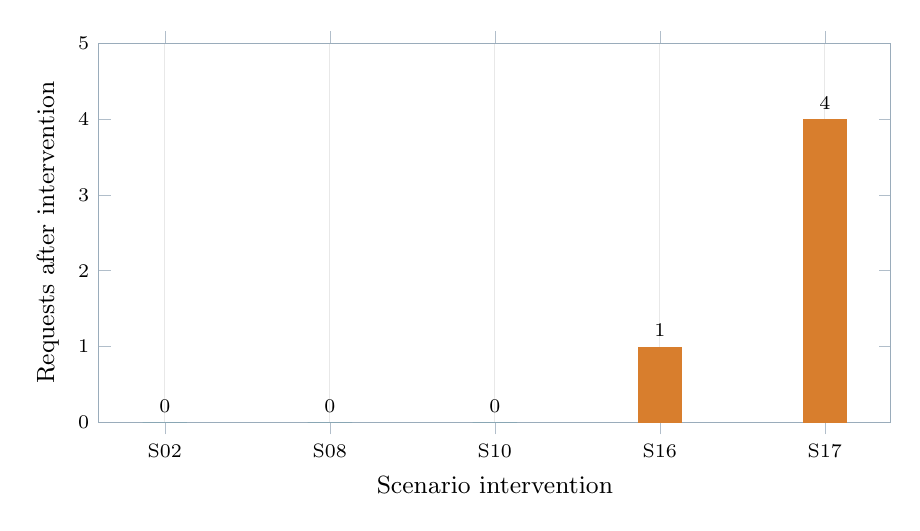
\begin{tikzpicture}
\begin{axis}[vgcplot,ybar,bar shift=0pt,bar width=16pt,width=.96\linewidth,height=6.4cm,ymin=0,ymax=5,ytick={0,1,2,3,4,5},xtick={0,1,2,3,4},xticklabels={S02,S08,S10,S16,S17},xlabel={Scenario intervention},ylabel={Requests after intervention},nodes near coords,point meta=y]
\addplot[fill=resultteal,draw=none] coordinates {(0,0)};
\addplot[fill=resultteal,draw=none] coordinates {(1,0)};
\addplot[fill=resultteal,draw=none] coordinates {(2,0)};
\addplot[fill=resultamber,draw=none] coordinates {(3,1)};
\addplot[fill=resultamber,draw=none] coordinates {(4,4)};
\end{axis}\end{tikzpicture}
\caption{Requests recorded after selected intervention boundaries, excluding each scenario's setup. S02: unchanged repair pass; S08: unselected context update; S10: equal selected content at a new context version; S16: architecture contract change repaired to equal API content; S17: tightened source clause followed by repair. These are different deterministic interventions, not matched performance benchmarks or samples of language-model cost.}\label{fig:request-deltas}
\end{figure}

\begin{table}[tbp]
\centering
\caption{Request counts around selected interventions. The cut index is the zero-based event position before the intervention; S02 cuts after its completed setup because its unchanged repair pass emits no new event. Values are read from recorded dispatch events.}\label{tab:request-interventions}
\footnotesize
\setlength{\tabcolsep}{3pt}
\renewcommand{\arraystretch}{1.13}
\begin{tabularx}{\linewidth}{@{}lXrrr@{}}\toprule
ID & Intervention & Cut & Before & After\\\midrule
S02 & No change & 8 & 4 & 0\\
S08 & Unselected context & 8 & 4 & 0\\
S10 & Equal content/version & 13 & 6 & 0\\
S16 & Equal API repair & 8 & 4 & 1\\
S17 & Tightened clause & 8 & 4 & 4\\
\bottomrule\end{tabularx}
\end{table}

Figure~\ref{fig:request-deltas} removes setup from a small set of interpretable change traces (Table~\ref{tab:request-interventions}). No relevant change, unselected context and a new version with equal selected content cause no additional request. Equal architecture output after a contract change requires the architecture's own new proposal but lets compatible descendants reuse evidence. Tightening the source clause reaches different implementation/verification observations despite an unchanged API, so the repair propagates. This is observed suppression of unnecessary calls in these fixtures. There is no full-regeneration baseline or provider token measurement, and these unequal interventions cannot establish a general speedup or cost-saving percentage.

\begin{table}[tbp]
\centering
\caption{Finite-language and recorded-execution checks. Domain sizes describe this restricted language; no sampling uncertainty is attached to exhaustive finite counts.}\label{tab:validation-domains}
\footnotesize
\setlength{\tabcolsep}{3pt}
\renewcommand{\arraystretch}{1.13}
\begin{tabularx}{\linewidth}{@{}Xrl@{}}\toprule
Check & Count & Interpretation\\\midrule
Typed policy tables, both settings & 8,192 & Exhaustive enumeration\\
Strict-policy event words, length 0--6 & 1,093 & All bounded words\\
Malformed table fixtures & 6 & Specific negative examples\\
Controller traces admitted & 28 & Recorded executions only\\
Corrupted traces rejected & 9 & Checker sensitivity\\
Transaction regression tests & 12 & Executed tests, not proof\\
\bottomrule\end{tabularx}
\end{table}

S28 has no controller transition events in Figure~\ref{fig:scenario-heatmap}: its work is exhaustive validation of the finite proposal language and bounded interpretation of event words. Its conforming empty controller trace does not supply evidence about the interpreter. That evidence instead comes from the dedicated oracle assertions summarized in Table~\ref{tab:validation-domains}, together with the separate mathematical argument and scoped policy lemmas. The bounded event-word campaign does not replace an unbounded interpreter refinement proof, and the malformed fixtures do not enumerate arbitrary malformed syntax.

\subsection{Regression coverage, trace-checker sensitivity and reproduction}

\begin{table}[tbp]
\centering
\caption{Individual transaction regressions and deliberately corrupted traces. OK denotes the expected outcome, including rejection of every corrupted trace; it is not a universal correctness verdict.}\label{tab:negative-controls}
\footnotesize
\setlength{\tabcolsep}{3pt}
\renewcommand{\arraystretch}{1.13}
\begin{tabularx}{\linewidth}{@{}lXl@{}}\toprule
Family & Check & Outcome\\\midrule
\multicolumn{3}{l}{\textit{Transaction regression tests}}\\
T01 & Primitive types and malformed rows & OK\\
T02 & Deletion/recreation request identity & OK\\
T03 & Duplicate cannot overwrite acceptance & OK\\
T04 & Unchanged-episode budget retention & OK\\
T05 & Forged publication token rejection & OK\\
T06 & Namespace injectivity / missing reference & OK\\
T07 & Mutable proposal alias isolation & OK\\
T08 & Publication on partial repair states & OK\\
T09 & Atomic reconfiguration rollback & OK\\
T10 & Mandatory views and structural reads & OK\\
T11 & Context suspension / reactivation & OK\\
T12 & Successful zero-match completion & OK\\
\midrule\multicolumn{3}{l}{\textit{Trace corruption controls}}\\
C01 & unknown action & Rejected\\
C02 & sequence gap & Rejected\\
C03 & counter & Rejected\\
C04 & provenance & Rejected\\
C05 & publication revision & Rejected\\
C06 & missing event & Rejected\\
C07 & acceptance source deletion & Rejected\\
C08 & acceptance context change & Rejected\\
C09 & acceptance contract change & Rejected\\
\bottomrule\end{tabularx}
\end{table}

The controls in Table~\ref{tab:negative-controls} target different boundaries: API transactions, structural admissibility, mutable aliases and replayed semantic events. In particular, acceptance events containing hidden source/context/contract changes must be rejected even when the proposed value itself is valid. These controls test sensitivity of the checker and the exercised implementation paths; they neither authenticate the log nor exclude omitted final suffixes or untested behaviors. A uniform pass column therefore records satisfaction of predefined expectations, not a confidence estimate for deployed reliability.

\begin{table}[tbp]
\centering
\caption{Inventory of archived domain-verification campaigns before this manuscript expansion. Pass/fail/inconclusive refer to whole-stage status. Inconclusive proof stages include successful scoped lemmas but an open central gate. Paper-build and tool-doctor invocations are excluded from experiment counts.}\label{tab:campaign-history}
\footnotesize
\setlength{\tabcolsep}{3pt}
\renewcommand{\arraystretch}{1.13}
\begin{tabularx}{\linewidth}{@{}Xrrrr@{}}\toprule
Campaign & Runs & Pass & Fail & Inconclusive\\\midrule
baseline & 1 & 0 & 0 & 1\\
case-study & 5 & 5 & 0 & 0\\
clean-reproduction & 2 & 2 & 0 & 0\\
conformance & 5 & 5 & 0 & 0\\
models & 4 & 4 & 0 & 0\\
mutations & 4 & 4 & 0 & 0\\
proofs & 4 & 0 & 0 & 4\\
spec-check & 3 & 3 & 0 & 0\\
tests & 5 & 5 & 0 & 0\\
witnesses & 2 & 2 & 0 & 0\\
\bottomrule\end{tabularx}
\end{table}

\begin{table}[tbp]
\centering
\caption{Clean extracted-directory reproductions of two packaged snapshots (ZIP SHA-256 prefixes identify them). A match compares the reported scientific outcomes; the incomplete baseline and proof stages are expected nonzero exits. Existing host tools and the pinned proof-container image are reused, so this is not a fresh-OS experiment.}\label{tab:clean-reproductions}
\footnotesize
\setlength{\tabcolsep}{3pt}
\renewcommand{\arraystretch}{1.13}
\begin{tabularx}{\linewidth}{@{}llrrl@{}}\toprule
Run & ZIP hash prefix & Files & Open stages & Outcomes\\\midrule
R1 & \texttt{8c54585b54} & 548 & 2 & Matched\\
R2 & \texttt{cee85e2b0c} & 557 & 2 & Matched\\
\bottomrule\end{tabularx}
\end{table}

Tables~\ref{tab:campaign-history} and~\ref{tab:clean-reproductions} prevent a polished final pass from erasing development failures or open obligations. The first proof trial's failed modules are retained explicitly in Table~\ref{tab:proof-development}; its whole-stage classification is inconclusive because the central proof gate remains unfinished. Historical baseline reproduction is also inconclusive because the cited original explorers were absent. The clean ZIP reproductions recover the same finite counts and scenario outcomes with those nonzero statuses intact. Repetition demonstrates procedural reproducibility on the recorded host environment; it supplies no independent samples for a significance test. The evidence supports guard debugging, scoped proof steps and conformance of recorded executions, while full parameterized safety, history-budget induction and action correspondence remain open.

\FloatBarrier
% END GENERATED DETAILED RESULTS

\section{Related work and formal-method choices}\label{sec:related}
\paragraph{Closest combination and concurrency foundation.} Stevens already connects software build, stamps, failures, and heterogeneous model consistency, proving soundness and incrementality for an extended build framework~\cite{megamodelbuild}. Our contribution is not that connection. We specify acceptance of asynchronous untrusted proposals under current contracts and authority, unsuccessful episode budgets, suspension, and configuration transactions. The atomic revalidation step is an application of optimistic concurrency control~\cite{occ}, rather than a new concurrency-control principle. The combined proof obligations identify what a generative coordinator must additionally preserve.

Shield synthesis supplies another close comparison: a synthesized shield corrects reactive outputs according to formal safety requirements~\cite{shield}. Our controller instead defers or rejects primitive proposals, preserves provenance under change, and may report terminal failure. We establish neither instantaneous corrective synthesis nor minimum-deviation shielding. The finite decision-table instance demonstrates how stronger behavioral claims become available with a sufficiently restricted proposal language.
\paragraph{Execution enforcement.} Schneider characterizes policies enforceable by execution monitoring~\cite{schneider}. Runtime enforcement further studies how monitors modify executions to ensure specified properties; Pinisetty et al. give a timed-property theory with explicit correctness criteria~\cite{pinisetty}. Our controller also excludes invalid steps, but its state includes persistent generated artifacts, dependency episodes, and transactional configuration. We use untimed guarded transitions because the target claims concern freshness and admissibility, not deadlines. A timed-automaton extension would be appropriate for bounded response latency, which is not established here.

\paragraph{Model transformation and consistency.} ATL provides typed transformation rules and explicit execution support~\cite{atl}. Stevens studies consistency across networks of heterogeneous models~\cite{stevens}, and Klare and Gleitze analyze termination and expressiveness of network execution strategies~\cite{klare}. These works make clear why pairwise consistency and global restoration cannot be conflated. Our setting uses directed, single-producer stages with nondeterministic primitive proposals. It does not establish the usual round-trip laws of bidirectional lenses (laws relating updates in opposite directions). The additional proof obligations concern rejected values, obsolete responses, and generation contracts.

\paragraph{Incremental computation and build systems.} Self-adjusting computation tracks dependencies and propagates changes~\cite{acar}; build-system theory separates scheduling from rebuilding~\cite{mokhov}. The observation signature is a rebuild key, and failed-attempt memory extends it with an explicit terminal unsuccessful outcome. Unlike deterministic rebuilding, two valid repairs may produce different primitive values. Our theorem therefore preserves admissibility and suppresses unnecessary calls relative to observations, rather than claiming equality with a fresh stochastic run. This distinction prevents importing deterministic incremental-correctness results without their hypotheses.

\paragraph{State-machine refinement and verification evidence.} IronFleet illustrates how state-machine refinement can connect protocol behavior to high-level specifications with mechanized implementation proofs~\cite{ironfleet}. We give a mathematical forward simulation at the coordination level; its full mechanization and implementation refinement remain open. Recent work in this journal supplies further methodological context: Grosen et al. give symbolic timed monitoring algorithms~\cite{grosen}; Lu et al. use scenarios to guide hybrid-network verification~\cite{lu}; Amilon et al. formalize correctness of program instrumentation~\cite{amilon}. Our use of untimed automata does not inherit their timed, hybrid, or instrumentation results.

Inductive invariants fit ownership and structural safety because each controller action has a local preservation obligation. Simulation fits asynchronous proposals because transport and request-delivery detail can be erased while budget increments and accepted effects remain visible. Dependency equality fits repair locality because it states exactly when cached validation evidence is reusable. Topological induction fits terminality because earlier stages stabilize before later stages execute. These techniques address different obligations; replacing all four with a state diagram would leave the main claims unsupported.

\section{Limitations and research obligations}\label{sec:limitations}
The trusted computing base, the components whose correct operation is assumed, contains normalization, signature construction, authorization, transaction isolation, validator execution, and publication. Bugs in any of these components can violate the assumptions. Recording provenance is not sufficient: the controller must enforce it at the write boundary. A concrete implementation should establish refinement to Section~\ref{sec:rules}, including durable request identifiers, crash recovery, and transaction serializability. The present paper supplies no end-to-end machine-checked implementation proof.

The semantics treats generated code as inert data. Publication releases a checked snapshot; execution requires the separately stated interpreter or deployment assumptions. Sandboxed execution of validators is an assumption, not a consequence of primitive-only writes. A worker with independent filesystem, network, or deployment permissions could create effects outside the machine. Such effects require mediated tool actions and a larger transition system. Likewise, append-only audit records support reconstruction only if storage and identity are trustworthy; traces establish recorded derivation, not causal understanding or originality of generated content.

Footprint adequacy is the principal semantic boundary. Engineers must show that selected observations include all information needed by the desired relation, including negative dependencies and shared context. Parsers and finite test suites often establish only weaker relations. Theorem~\ref{thm:table} discharges this obligation for one finite language. A compositional route to stronger claims is to require proof-carrying proposals checked by a trusted verifier and to express interface assumptions explicitly. Whether that is practical for a given artifact language requires further research and cannot be inferred from successful generation.

The acyclic discipline limits feedback and shared mutable targets. It defines the base usability semantics and supports the terminality proof, while excluding unrestricted collaborative editing and cyclic consistency restoration. Global conflict is reported after local repair; no theorem promises an automatic solution. Observations and input revisions can grow without bound, and the bounded model checks do not establish scalability. Empirical performance claims or a broader implementation evaluation would need independent workloads, declared fault models, reproducible measurements, and baselines matched on context and validation strength.

\Needspace{16\baselineskip}
\section{Conclusion}
A deterministic controller with ranked acyclic dependencies can coordinate untrusted generative proposals with explicit, conditional guarantees. Typed structural normalization protects object and reference integrity; exact effective signatures and atomic commitment exclude obsolete results; publication separates local acceptance from global consistency. Dependency episodes give an honest generation bound, and a finite acyclic discipline yields a terminal success-or-failure verdict after inputs stabilize. Transactional reconfiguration preserves these properties when its proof obligations are checked. The central remaining obligations are the full parameterized safety and history-budget mechanization, checked asynchronous-to-atomic action correspondence, general semantic footprint adequacy and validator soundness, and refinement of a concrete implementation to the controller machine.

\section*{Statements and Declarations}
\paragraph{Research materials and data.} This study supplies mathematical semantics, scoped proof artifacts, bounded model checks and scripted reference-controller scenarios. No real-model performance or unrestricted generated-code correctness measurements are claimed. Sources, raw reports, independent expectations and reproduction commands are supplied locally; no public archive identifier has been assigned. The full parameterized controller and refinement proof gates remain incomplete.
\paragraph{AI assistance.} Generative AI assisted development of the formalization, prose, executable exploration, and internal critical reviews. The reviews are simulated research assistance and do not constitute independent human peer review. The human author is responsible for checking the claims, proofs, references, and final submission.
\paragraph{Funding and competing interests.} Funding and competing-interest declarations must be confirmed by the author before submission; no declaration about undisclosed circumstances is made here.

\begingroup
\setlength{\bibsep}{0.5em}
\interlinepenalty=10000
\bibliography{references}
\endgroup
\end{document}
